\chapter{Operads}
\section{Operads on Sets}

Let $Y, Z$ be sets. Consider a function $g: Y \to Z$. The way we've been 
taught to think about this function is as a process where we're 
sending an element $y \mapsto g(y)$ 
in a well-defined manner. 
\begin{center}
    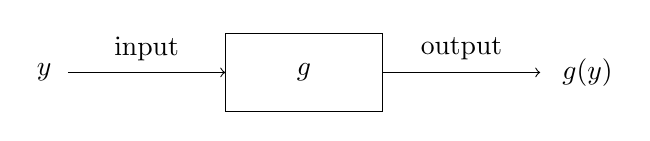
\begin{tikzpicture}
        \draw (0,0.5) rectangle (2,1.5);
        \node at (1,1) {$g$};
        \node at (-2.3, 1) {$y$};
        \node at (4.6, 1) {$g(y)$};
        \draw[->] (-2,1) -- (0,1);
        \draw[->] (2,1) -- (4,1);
        \node at (-1, 1.3) {input};
        \node at (3, 1.3) {output};
    \end{tikzpicture}
    
    \emph{The typical picture one uses when describing a function.}
\end{center} 

Furthermore, if we have another function $f: X \to Y$, 
then we can set up a pipeline $x \mapsto f(x) \mapsto g(f(x))$. This then 
establishes an obvious function $g \circ f: X \to Z$. 
\begin{center}
    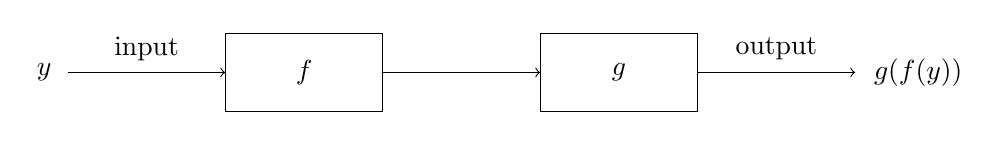
\begin{tikzpicture}
        \draw (0,0.5) rectangle (2,1.5);
        \draw (4,0.5) rectangle (6,1.5);
        
        \node at (1,1) {$f$};
        \node at (5,1) {$g$};
        \node at (-2.3, 1) {$y$};
        \node at (8.8, 1) {$g(f(y))$};

        \draw[->] (-2,1) -- (0,1);
        \draw[->] (2,1) -- (4,1);
        \draw[->] (6,1) -- (8, 1); 


        \node at (-1, 1.3) {input};
        \node at (7, 1.3) {output};
    \end{tikzpicture}

    \emph{The function $g \circ f$.}
\end{center}

But the way that we've thought about functions, and more generally morphisms,
is actually over-simplistic. Here we will demonstrate that we can \emph{generalize 
the concept of morphism composition}.

Denote $\aend_n(X)$ to be the set of all functions 
$f:X^n \to X$. Then for such a function, if we stick with our simplistic concept of plugging things in, we 
imagine something like
\begin{center}
    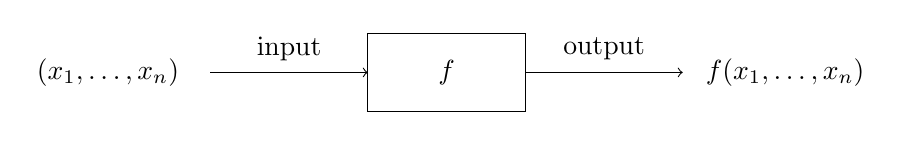
\begin{tikzpicture}
        \draw (0,0.5) rectangle (2,1.5);
        \node at (1,1) {$f$};
        \node at (-3.3, 1) {$(x_1, \dots, x_n)$};
        \node at (5.3, 1) {$f(x_1, \dots, x_n)$};
        \draw[->] (-2,1) -- (0,1);
        \draw[->] (2,1) -- (4,1);
        \node at (-1, 1.3) {input};
        \node at (3, 1.3) {output};
    \end{tikzpicture}
\end{center} 

However, a more natural way is to imagine that we're taking values 
$n$-many values $x_i \in X$ and plugging them into the function $f: X^n \to X$. 
That is, we don't have to just think of \emph{one} $g: Y \to X^n$ to form a concept of 
composition. We can instead imagine that each of these $x_i$ values came 
from functions $g_1: Y_1 \to X$, $g_2: Y_2 \to X, \cdots, g_n: Y_n \to X$. 
\begin{center}
    \begin{tikzcd}[column sep = 0.7cm, row sep = 0.9cm]
        Y_1
        \arrow[dr, swap, "g_1", near start, start anchor = {[xshift = -0.3cm]}, end anchor = {[xshift=-1cm]}]
        &[-1cm] 
        Y_2 \phantom{m}\cdots
        \arrow[d, "g_2", start anchor = {[xshift = -0.4cm]}, end anchor = {[xshift=-0.4cm]}]
        &[-1cm]
        Y_n \arrow[dl, near start, "g_n", start anchor = {[xshift = 0.3cm]}, end anchor = {[xshift=1cm]}]
        \\
        & X \times X \times \cdots \times X 
        \arrow[d, "f"]
        &\\
        & X & 
    \end{tikzcd}
\end{center}
This is in its own right a function; a function from $Y_1 \times Y_2 \times Y_n \to X$.
It's a generalization of function composition; when we only have one $g_1$ we just 
get back our original notion of function composition. We've been restricting ourselves this whole time.
Now to make this even more interesting, suppose $Y_1 = X^{a_1}, Y_2 = X^{a_2}, \dots, Y_n = X^{a_n}$
where $a_1, a_2, \dots, a_n$ are positive integers. That is, suppose we have that $g_i \in \aend_{a_i}(X)$. 
\begin{center}
    \begin{tikzcd}[column sep = 0.7cm, row sep = 0.9cm]
        X^{a_1}
        \arrow[dr, swap, "g_1", near start, start anchor = {[xshift = -0.3cm]}, end anchor = {[xshift=-1cm]}]
        &[-1cm] 
        X^{a_2} \phantom{m}\cdots
        \arrow[d, "g_2", start anchor = {[xshift = -0.4cm]}, end anchor = {[xshift=-0.4cm]}]
        &[-1cm]
        X^{a_n} \arrow[dl, near start, "g_n", start anchor = {[xshift = 0.3cm]}, end anchor = {[xshift=1cm]}]
        \\
        & X \times X \times \cdots \times X 
        \arrow[d, "f"]
        &\\
        & X & 
    \end{tikzcd}
\end{center}
The above composition can be expressed as $f(g_1, g_2, \dots, g_n)$ which we may  
denote as
\[
    f \circ_{a_1, a_2, \dots, a_n}(g_1, g_2, \dots, g_n): X^{a_1}\times X^{a_2}\times \cdots \times X^{a_n} \to X.
\]
and note that we've construction a function in $\aend_{a_1 + a_2 + \cdots + a_n}(X)$ using
one $f \in \aend_n(X)$ and $n$-many $g_i \in \aend_i(X)$. 
Then what we see is that our composition map is really a function that can be written formally as 
\[
    \circ_{a_1, a_2, \dots, a_n}: X^n \times (X^{a_1}\times X^{a_2}\times \cdots \times X^{a_n})
    \to 
    X^{a_1 + a_2 + \cdots + a_n} 
\]
Then we can make this even more interesting. Each $g_i: X^{a_i} \to X$ is \emph{just like} $f: X^n \to X$.
Hence we can repeat the same process on each $g_i$, and plug a family of functions $h_{i, j}: X^{k_{i,j}}\to X$
where $j = 1, 2, \dots, a_i$. 
\begin{center}
    \begin{tikzcd}[column sep = 0.7cm, row sep = 0.9cm]
        X^{k_{1,1}},
        \hspace{0.3cm}
        X^{k_{1,2}},
        \dots,
        \hspace{0.3cm}
        X^{k_{1,a_1}}
        \arrow[d, swap, "h_{1,1}", start anchor = {[xshift = -1.4cm]}, end anchor = {[xshift=-1.4cm]}]
        \arrow[d, "h_{1,2}",start anchor = {[xshift = -0.6cm]}, end anchor = {[xshift=-0.6cm]}]
        \arrow[d, "h_{1,a_1}",start anchor = {[xshift = 1.4cm]}, end anchor = {[xshift=1.4cm]}]
        &
        X^{k_{2,1}},
        \hspace{0.3cm}
        X^{k_{2,2}},
        \dots,
        \hspace{0.3cm}
        \arrow[d, swap, "h_{2,1}", start anchor = {[xshift = -2.2cm]}, end anchor = {[xshift=-2.2cm]}]
        \arrow[d, "h_{2,2}",start anchor = {[xshift = -1.2cm]}, end anchor = {[xshift=-1.2cm]}]
        \arrow[d, "h_{2,a_2}",start anchor = {[xshift = 0.7cm]}, end anchor = {[xshift=0.7cm]}]
        X^{k_{2,a_2}}
        \hspace{0.3cm}\cdots
        &
        X^{k_{n,1}},
        \hspace{0.3cm}
        X^{k_{n,2}},
        \dots,
        \hspace{0.3cm}
        X^{k_{1,a_n}}
        \arrow[d, swap, "h_{n,1}", start anchor = {[xshift = -1.4cm]}, end anchor = {[xshift=-1.4cm]}]
        \arrow[d, "h_{n,2}",start anchor = {[xshift = -0.6cm]}, end anchor = {[xshift=-0.6cm]}]
        \arrow[d, "h_{n,a_n}",start anchor = {[xshift = 1.4cm]}, end anchor = {[xshift=1.4cm]}]
        \\
        X\times X\times \hspace{-0.2cm} \overbracket[0.5pt][0.1cm]{\cdots}^{a_1\text{-times}} \hspace{-0.2cm} \times X
        \arrow[dr, swap, "g_1", near start, start anchor = {[xshift = -0.3cm]}, end anchor = {[xshift=-1cm]}]
        &[-1cm] 
        X\times X\times \hspace{-0.2cm} \overbracket[0.5pt][0.1cm]{\cdots}^{a_2\text{-times}} \hspace{-0.2cm} \times X
        \arrow[d, "g_2"]% start anchor = {[xshift = -0.4cm]}, end anchor = {[xshift=-0.4cm]}]
        \hspace{1cm}\cdots
        &[-1cm]
        X\times X\times \hspace{-0.2cm} \overbracket[0.5pt][0.1cm]{\cdots}^{a_n\text{-times}} \hspace{-0.2cm} \times X
        \arrow[dl, near start, "g_n", start anchor = {[xshift = 0.3cm]}, end anchor = {[xshift=1cm]}]
        \\
        & X \times X \times \cdots \times X 
        \arrow[d, "f"]
        &\\
        & X & &
    \end{tikzcd}
\end{center}
Now there are two ways to think about this function. There is 
\[
    [f \circ_{a_1, a_2, \dots, a_n} (g_1, g_2, \dots, g_n)]\circ_{k_{1,1}, \dots, k_{1, a_1}, \dots, k_{n, a_1}, \dots, k_{n, a_n}}(h_{1,1}, \dots, h_{n, a_n})
\]  
which first composes $f$ with the $g$-family, and then composes with the $h$-family, and then there is 
\[
    f \circ_{(k_{1,1}+ \cdots + k_{1, a_1}), \dots, (k_{n, 1}+ \cdots + k_{n, a_n})}
    \big(g_1 \circ_{k_{1,1}, \dots, k_{1, a_1}}(h_{1,1}, \dots, h_{1, a_1}), \dots, g_n \circ_{k_{n, 1}, \dots, k_{n, a_n}}(h_{n,1}, \dots, h_{n, a_n})\big)
\]
which first composes each $g$ with its respective $h$-family, and then composing the resulting
structure with $f$. Since these are just functions, and individual composition is associative, 
the above two ways are the same. This construction which we have demonstrated is an example
of an \emph{operad}; specifically, a symmetric operad.
The previous example can now be seen as motivation for the following two
definitions (which will definitely need repeated read-overs).

\begin{definition}
    A \textbf{nonsymmetric operad} $X$ in \textbf{Set} consists of 
    a family of sets $\{X_n\}_{n=1}^{\infty}$, an identity element $I \in X_1$ (whose purpose will soon be elaborated),
    and a composition map 
    \begin{align*}
        \circ_{n, a_1, a_2, \dots, a_n}: X_n \times (X_{a_1} \times X_{a_2}\times \cdots \times X_{a_n}) \to X_{a_1 + a_2 + \cdots + a_n}\\
        (f, g_1, g_2, \dots, g_n) \mapsto f\circ_{a_1, a_2, \dots, a_n} (g_1, g_2, \dots, g_n)
    \end{align*}
    which must exist for each $n = 1, 2, \dots$, and any $a_1, a_2, \dots, a_n \in \mathbb{N}$, 
    such that
    \begin{description}
        \item[(NS-OP1: Associativity.) ] Let $n \in \mathbb{N}$ and consider $f \in X_n$. 
        Let $a_1, a_2 \dots, a_n \in \mathbb{N}$. Then  
        \begin{gather*}
            [f \circ_{a_1, a_2, \dots, a_n} (g_1, g_2, \dots, g_n)]\circ_{k_{1,1}, \dots, k_{1, a_1}, \dots, k_{n, a_1}, \dots, k_{n, a_n}}(h_{1,1}, \dots, h_{n, a_n})\\
            =\\
            f \circ_{(k_{1,1}+ \cdots + k_{1, a_1}), \dots, (k_{n, 1}+ \cdots + k_{n, a_n})}
    \big(g_1 \circ_{k_{1,1}, \dots, k_{1, a_1}}(h_{1,1}, \dots, h_{1, a_1}), \dots, g_n \circ_{k_{n, 1}, \dots, k_{n, a_n}}(h_{n,1}, \dots, h_{n, a_n})\big)
        \end{gather*}
        \item[(NS-OP2): Identity.] For every $f \in X_n$ we have that 
        \[
            f \circ_{1, 1, \dots, 1} (I, I, \dots, I) = f = I \circ_n (f).
        \]   
    \end{description}
\end{definition}

\begin{definition}
    A \textbf{symmetric operad} is a nonsymmetric operad $X$ with a 
    right group action $\cdot_n: X_n \times S_n \to X_n$
    by the symmetric group $S_n$
    for each $n = 1, 2, \dots$, subject to the following axioms. 
    \begin{description}
        \item[(S-OP1: Equivariance 1)]
        Let $f \in X_n$ and pick $g_{1} \in X_{a_1}, \dots, g_n \in X_{a_n}$ for 
        some $a_1, a_2, \dots, a_n \in \mathbb{N}$. Then for a $\tau \in S_n$, we must 
        have 
        \[
            (f \cdot \tau)\circ_{a_1, \dots, a_n}(g_1, \dots, g_n)
            =
            (f \circ_{a_{\tau^{-1}(1)}, \dots, a_{\tau^{-1}(n)}}(g_{\tau^{-1}(1)}, \dots, g_{\tau^{-1}(n)}))\cdot \tau'
        \]
        where $\tau' \in S_{a_1 + \cdots + a_n}$. Here, $\tau'$ is a \emph{block permutation} 
        that swaps the $i$-th block with the $\tau(i)$-th block. That is, if 
        $\tau \in S^n$ as a permutation acts as 
        \[
            (1, 2, \dots, n) \mapsto (\tau(1), \tau(2), \dots, \tau(n))
        \]
        then $\tau' \in S_{a_1 + a_2 + \cdots + a_n}$ acts as 
        \begin{gather*}
            (\overbrace{\textcolor{Red}{1, 2, \dots, a_1}}^{\text{1st block}}, \dots, 
            \overbrace{\textcolor{Green}{a_1 + \cdots + a_i+1, \dots a_1 + \cdots + a_{i+1}}}^{i\text{-th block}}, \dots
            \overbrace{\textcolor{RoyalBlue}{a_1 + \cdots + a_{n-1}+ 1, \dots, a_1 + \cdots + a_n}}^{n\text{-th block}})\\
            \mapsto\\
            (\dots, \overbrace{\textcolor{Red}{1, 2, \dots, a_1}}^{\tau(1)\text{-th block}}, \dots 
            ,  \overbrace{\textcolor{Green}{a_1 + \cdots + a_i+1, \dots, a_1 + \cdots + a_{i+1}}}^{\tau(i)\text{-th block}}, \dots
            ,  \overbrace{\textcolor{RoyalBlue}{a_1 + \cdots +  a_{n-1}+1, \dots, a_1 + \cdots + a_{n}}}^{\tau(n)\text{-th block}}, \dots
            ).
        \end{gather*}

        \item[(S-OP2: Equivariance 2)]  
        Let $f, g_i$ is as above, and choose $\sigma_1 \in S_1, \dots, \sigma_{n} \in S_n$. 
        Then we have that 
        \[
            f \circ_{a_1, \dots, a_n}(g_1 \cdot \sigma_1, \dots, g_n \cdot \sigma_n)
            =
            (f \circ_{a_1, \dots, a_n}(g_1, \dots, g_n))\cdot (\sigma_1, \dots,\sigma_n)
        \]
        where $(\sigma_1, \sigma_2, \dots, \sigma_n) \in S_{a_1 + a_2 + \cdots + a_n}$ 
        is the permutation described as below. 
        \begin{gather*}
            (\overbrace{\textcolor{Red}{1, 2, \dots, a_1}}^{\text{1st block}}
            ,\dots,
            \overbrace{\textcolor{RoyalBlue}{a_1 + \cdots + a_{n-1}+ 1,, \dots, a_1 + \cdots + a_{n-1}a_n}}^{n\text{-th block}} )
            \\
            \mapsto\\
            (\underbrace{\sigma_1(\textcolor{Red}{1}), \sigma_1(\textcolor{Red}{2}), \dots, \sigma_1(\textcolor{Red}{a_1})}_{\text{1st block}}, 
            \dots, 
            % \overbrace{
            % \textcolor{Green}{a_1 + \cdots + a_i+}    
            % \sigma_i(\textcolor{Green}{1})}^{(a_i+1)\text{-th entry}}, 
            % \sigma_i(\textcolor{Green}{2}), \dots, \sigma_i(\textcolor{Green}{a_i})
            % \dots, 
            \underbrace{\textcolor{RoyalBlue}{a_1 + \cdots +  a_{n-1}+}
            \sigma_n(\textcolor{RoyalBlue}{1}), 
            \dots, \textcolor{RoyalBlue}{a_1 + \cdots +  a_{n-1}+}\sigma_n(\textcolor{RoyalBlue}{a_n})
            }_{n\text{-th block}}
            )
        \end{gather*}
    \end{description}
\end{definition}

\begin{example}
    We can continue with our previous construction concerning 
    the family of sets 
    \[
        \aend_n(X) = \{f: X^n \to X \mid f \in \textbf{Set}\}
    \]
    to demonstrate that it 
    forms a symmetric operad. As we already established associativity \textbf{NS-OP1}, we need 
    to verify the identity axiom \textbf{NS-OP2}. Such an identity element can be chosen if 
    we select $I = 1_X: X \to X$. On one hand we have for any $f \in X^n$ that
    \[
        f \circ_{1, 1, \dots, 1}(I, I, \dots, I) = f(1_x, 1_x, \dots, 1_x) = f
    \]
    while on the other we have that $I \circ_n f = 1_X \circ f = f$. 
    Next, define a group action of $S_n$ on $\aend_n(X)$ as 
    \[
        (f \cdot \sigma)(x_1, x_2, \dots, x_n) = f(x_{\sigma(1)}, x_{\sigma(2)}, \dots, x_{\sigma(n)}).
    \]
    We now verify \textbf{S-OP1} with this group action. 
    Let $f \in \aend_n(X)$ and $g_i \in \aend_i(X)$ for $i = 1, 2, \dots, n$.
    For a given $\tau \in S_n$, consider the points $(x_1, \dots, a_1) \in X^{a_1}, \dots, (x_1, \dots, a_n) \in X^{a_n}$.
    Observe that $(f \cdot \tau) \circ_{a_1, \dots, a_n}(g_1, \dots, g_n)$ first plugs in 
    the each $(x_{a_{i}-1}, \dots, x_{a_i})$ into $g_i$, which is then 
    plugged into $f$. However, the action of $\tau$ swaps these resulting coordinates. 
    Thus we get that 
    \[
        (f \cdot \tau) \circ_{a_1, \dots, a_n}(g_1, \dots, g_n)(x_1, \dots, a_1, \dots, x_{a_{n-1}+1}, \dots, x_{a_n})
        = 
        (\dots, \overbrace{g_i(x_{a_{i-1}+1}, \dots, x_{a_i})}^{\tau(i)-\text{th entry}}, \dots )
    \]
    How do we write this more formally? Well, to answer that, we need to know the answer 
    to the following question: which $g_i(x_{a_{i-1}+1}, \dots, x_{a_i})$
    maps to, say, the 1st coordinate? This is equivalently to asking: what is $\tau^{-1}(1)$? 
    Hence we see that 
    \begin{gather*}
        (f \cdot \tau) \circ_{a_1, \dots, a_n}(g_1, \dots, g_n)(x_1, \dots, a_1, \dots, x_{a_{n-1}+1}, \dots, x_{a_n})\\
        =
        f(g_{\tau^{-1}(1)}(x_{a_{\tau^{-1}(1)-1}+1}, \dots, x_{a_{\tau^{-1}(1)}}), \dots, g_{\tau^{-1}(n)}(x_{a_{\tau^{-1}(n)-1}+1}, \dots, x_{a_{\tau^{-1}(n)}}))\\
        = 
        f \circ_{\tau^{-1}(1), \tau^{-1}(2), \dots, \tau^{-1}(n)}(g_{\tau^{-1}(1)}, g_{\tau^{-1}(2)}, \dots, g_{\tau^{-1}(n)})
        (x_{a_{\tau^{-1}(1)-1}+1}, \dots, x_{a_{\tau^{-1}(1)}}, \dots, x_{a_{\tau^{-1}(n)-1}+1}, \dots, x_{a_{\tau^{-1}(n)}})\\
        =
        \Big(f \circ_{\tau^{-1}(1), \tau^{-1}(2), \dots, \tau^{-1}(n)}(g_{\tau^{-1}(1)}, g_{\tau^{-1}(2)}, \dots, g_{\tau^{-1}(n)}) \cdot \tau'\Big)(x_1, \dots, x_{a_1}, \dots, x_{a_{n-1}+1}, \dots, x_{a_n}).
    \end{gather*}
    where $\tau'$ is the block permutation described in the definition. 
    Thus we see that 
    \[
        (f \cdot \tau) \circ_{a_1, \dots, a_n}(g_1, \dots, g_n)
        =
        f \circ_{\tau^{-1}(1), \tau^{-1}(2), \dots, \tau^{-1}(n)}(g_{\tau^{-1}(1)}, g_{\tau^{-1}(2)}, \dots, g_{\tau^{-1}(n)}) \cdot \tau'
    \]
    as desired. Thus we have \textbf{S-OP1}. Finally, we show \textbf{S-OP2}, which 
    is a bit easier to demonstrate. As before, let $f, a_i$ and $g_i$ be as described 
    before. Let $\sigma_1 \in S_1, \dots, \sigma_n \in S_n$. 
    Then 
    \begin{gather*}
        f \circ_{a_1, \dots, a_n}(g_1 \cdot \sigma_1, \dots, g_n \cdot \sigma_n)(x_1, \dots, x_{a_1}, \dots, x_{a_{n-1}+1}, \dots, x_{a_n})\\
        =
        f\Big( (g_1 \cdot \sigma_1)(x_1, \dots, x_{a_1}), \dots, (g_n \cdot \sigma_n)(x_{a_{n-1}+1}, \dots, x_{a_n})  \Big)\\
        =
        f\Big( g_1(x_{\sigma_1(1)}, \dots, x_{\sigma_1(a_1)}), \dots, g_n(x_{\sigma_n(1)}, \dots, x_{\sigma_n(a_n)}) \Big)\\
        = 
        \Big( f \circ_{a_1, \dots, a_n}(g_1, \dots, g_n) \Big)(x_{\sigma_1(1)}, \dots, x_{\sigma_1(a_1)}, \dots, x_{\sigma_n(1)}, \dots, x_{\sigma_n(a_n)})\\
        = 
        \Big( f \circ_{a_1, \dots, a_n}(g_1, \dots, g_n) \Big) \cdot (\sigma_1, \dots, \sigma_n)(x_1, \dots, x_{a_1}, \dots, x_{a_{n-1}+1}, \dots, x_{a_n})
    \end{gather*}
    Thus we see that 
    \[
        f \circ_{a_1, \dots, a_n}(g_1 \cdot \sigma_1, \dots, g_n \cdot \sigma_n)
        =(f \circ_{a_1, \dots, a_n}(g_1, \dots, g_n)) \cdot (\sigma_1, \dots, \sigma_n)
    \]
    so that \textbf{S-OP2} is satisfied. 
    All together, we have that for any set $X$, the family of sets $\aend_{n}(X)$ 
    forms a symmetric operad.
\end{example}

\begin{example}
    Consider the family of sets $\text{Assoc}_n = S_n$ where each level 
    is the $n$-th symmetric group. Suppose that $\tau \in S_n$ and 
    that $\sigma_1 \in S_{a_1}, \sigma_2 \in S_{a_2}, \dots, \sigma_n \in S_{a_n}$
    for $a_1, a_2, \dots, a_n \in \mathbb{N}$. Then we define 
    \[
        \tau \circ_{a_1, \dots, a_n}(\sigma_1, \sigma_2, \dots, \sigma_n) \in S_{a_1 + a_2 + \cdots + a_n}   
    \]
    as a permutation of $a_1 + a_2 + \cdots + a_n$ letters. Before we describe the permutation, we'll
    introduce some notation. Consider the (ordered) tuple of the first $a_1 + \cdots + a_n$ integers. 
    \[
        (\textcolor{Red}{1, 2, \dots, a_1}, 
        \textcolor{Green}{a_1 + 1, a_1 + 2, \dots, a_1 + a_2},
        \dots
        \textcolor{RoyalBlue}{(a_{1} + \cdots + a_{n-1})+1, \dots, (a_{1} + \cdots + a_{n-1}) + a_n})
    \]
    We can more compactly denote this tuple as 
    \[
        (\textcolor{Red}{1, 2, \dots, a_1},
        \textcolor{Green}{1', 2', \dots, a'_2}, 
        \dots, 
        \textcolor{RoyalBlue}{1', 2', \dots, a'_n}) 
    \]
    where from either context or coloring it will be clear what each $1', 2',\dots$ 
    indicates. For example, above we'll have that 
    $\textcolor{Green}{1' = a_1 + 1}$ and $\textcolor{Green}{2' = a_1+ 2}$ 
    wheres 
    $\textcolor{RoyalBlue}{1' = (a_1 + \cdots + a_{n-1}) + 1}$ and $\textcolor{RoyalBlue}{2' = (a_1 + \cdots + a_{n-1}) + 2}$.
    With that said, we can define $\tau \circ_{a_1, \dots, a_n}(\sigma_1, \sigma_2, \dots, \sigma_n) \in S_{a_1 + a_2 + \cdots + a_n}$
    by its action on such a tuple, pictured below. 
    \begin{center}
        \begin{tikzcd}[column sep = 1.4cm, row sep = 0.7cm]
            (\textcolor{Red}{1, 2, \dots, a_1},
            \textcolor{Green}{1', 2', \dots, a'_2}, 
            \dots, 
            \textcolor{RoyalBlue}{1', 2', \dots, a'_n}) 
            \arrow[d, "\sigma_1", start anchor = {[xshift = -3.5cm]}, end anchor = {[xshift=-3.5cm]}]
            \arrow[d, "\sigma_2", start anchor = {[xshift = -1.4cm]}, end anchor = {[xshift=-1.4cm]}]
            \arrow[d, draw = none, start anchor = {[xshift = 1cm]}, end anchor = {[xshift=1cm]}, "\raisebox{+0.2ex}{\dots}" description]
            \arrow[d, "\sigma_n", start anchor = {[xshift = 2.7cm]}, end anchor = {[xshift=2.7cm]}]
            \\
            (\underbrace{\sigma_1(\textcolor{Red}{1}), \sigma_1(\textcolor{Red}{2})), 
            \dots \sigma_1(\textcolor{Red}{a_1})}_{\text{1st block}}, 
            \underbrace{\sigma'_1(\textcolor{Green}{1}), \sigma'_1(\textcolor{Green}{2})), 
            \dots \sigma'_1(\textcolor{Green}{a_1})}_{\text{2nd block}}, \dots, 
            \underbrace{\sigma'_n(\textcolor{RoyalBlue}{1}), \sigma'_n(\textcolor{RoyalBlue}{2}) \dots, \sigma'_n(\textcolor{RoyalBlue}{a_n})}_{a_n\text{-th block}})
            \arrow[d, "\tau"]
            \\
            (\dots, \underbrace{\sigma_1(\textcolor{Red}{1}), \sigma_1(\textcolor{Red}{2})), 
            \dots \sigma_1(\textcolor{Red}{a_1})}_{\tau(1)\text{-th block}}, \dots, 
            \underbrace{\sigma'_1(\textcolor{Green}{1}), \sigma'_1(\textcolor{Green}{2})), 
            \dots \sigma'_1(\textcolor{Green}{a_1})}_{\tau(2)\text{-th block}}, \dots, 
            \underbrace{\sigma'_n(\textcolor{RoyalBlue}{1}), \sigma'_n(\textcolor{RoyalBlue}{2}), \dots, \sigma'_n(\textcolor{RoyalBlue}{a_n})}_{\tau(a_n)\text{-th block}}, \dots, )
        \end{tikzcd}
    \end{center} 
    which can be rewritten more formally as 
    \[
        (\overbrace{\sigma'_{\tau^{-1}(1)}(1), \sigma'_{\tau^{-1}(1)}(2), \dots, \sigma'_{\tau^{-1}(1)}(a_{\tau^{-1}(1)})}^{1\text{st block}}, 
        \dots, 
        \overbrace{\sigma'_{\tau^{-1}(n)}(1), \sigma'_{\tau^{-1}n}(2), \dots, \sigma'_{\tau^{-1}(n)}(a_{\tau^{-1}(n)})}^{n\text{-th block}} )
        \in 
        S_{a_1 + \cdots + a_n}.
    \]
    Now for each $\sigma_i \in S_{a_i}$, let $\rho_{i, j} \in S_{k_{i,j}}$ 
    for $j = 1, 2, \dots, a_i$ and for $k_{i,j} \in \mathbb{N}$. 
    For notational convenience, denote $K = k_{1,1}+ \cdots + k_{1,a_1}+ \cdots + k_{n,1} + \cdots + k_{n, a_n}$. 
    By our above definition, we can construct a permutation in $S_{K}$
    by composing $\tau$ with the $\sigma$-family and with the $\rho$-family.
    There are two possible ways to construct such a permutation 
    (and we'll show 
    that they are equivalent, therefore satisfying \textbf{NS-OP1}). 
    But before we do that 
    we must consider the first $K$ integers. 
    This will be a \emph{huge} tuple; in full notation this is
    \begin{center}
        \begin{tikzcd}
            \Big(
            \overbrace{
            \textcolor{Red}{1,2,\dots,k_{1,1}}}^{1\text{st block}},
            \overbrace{\textcolor{Orange}{k_{1,1}+1, k_{1,1} +2, \dots, k_{1,1}+k_{1,2}}}^{2\text{nd block}},\dots\\
            \dots
            \overbrace{\textcolor{Green}{(k_{1,1} + k_{1,2} + \cdots + k_{1, a_{1}-1})+1,
            (k_{1,1} + k_{1,2} + \cdots + k_{1, a_{1}-1})+2,
            \dots,
            (k_{1,1} + k_{1,2} + \cdots + k_{1, a_1-1}) + k_{1,a_1}}}^{a_1\text{-th block}}
            \dots
            \\
            \dots 
            \overbrace{
            \textcolor{Purple}{\displaystyle{\sum_{i=1}^{n-1}\sum_{j=1}^{a_i}k_{i, j}} + 1
            \displaystyle{\sum_{i}^{n-1}\sum_{j=1}^{a_i}k_{i, j}} + 2, 
            \dots, 
            \displaystyle{\sum_{i}^{n-1}\sum_{j=1}^{a_i}k_{i, j}} + k_{n, 1}}}^{(a_1 + a_2 + \cdots + a_{n-1}+1)\text{-th block}},
            \dots
            \\
            \dots, 
            \overbrace{
            \textcolor{RoyalBlue}{\displaystyle{\sum_{i}^{n-1}\sum_{j=1}^{a_i}k_{i, j}} + (k_{n, 1} + \cdots + k_{n, (a_n-1)})
            + 1,
            \displaystyle{\sum_{i}^{n-1}\sum_{j=1}^{a_i}k_{i, j}} + (k_{n, 1} + \cdots + k_{n, (a_n-1)})
            + 2,
            \dots, 
            \displaystyle{\sum_{i}^{n}\sum_{j=1}^{a_i}k_{i, j}}} }^{(a_1 + a_2 + \cdots + a_{n-1}+ a_n)\text{-th block}}
            \Big)
        \end{tikzcd}
    \end{center}
    Using our previous notation we can rewrite this as 
    \[
        (
        \overbrace{\textcolor{Red}{1, 2, \dots, k_{1,1}}}^{1\text{st block}}, 
        \overbrace{\textcolor{Orange}{1'}, 
        \textcolor{Orange}{2'}, \dots, \textcolor{Orange}{k_{1,2}}}^{2\text{nd block}}, 
        \dots, 
        \overbrace{\textcolor{Green}{1'}, \textcolor{Green}{2'}, \dots, \textcolor{Green}{k_{1, a_1}}}^{a_1\text{-th block}},
        \dots,
        \hspace{-0.5cm}
        \overbrace{\textcolor{Purple}{1'}, \textcolor{Purple}{2'}, \dots, \textcolor{Purple}{k_{n, 1}}}^{(a_1 + \cdots + a_{n-1}+1)\text{-th block}}
        \hspace{-0.5cm}
        ,\dots,
        \overbrace{\textcolor{RoyalBlue}{1'}, \textcolor{RoyalBlue}{2'}, \dots, \textcolor{RoyalBlue}{k_{n, a_n}}}^{(a_1 + \cdots + a_n)\text{-th block}}
        )
    \]
    where again, for example, $\displaystyle \textcolor{Orange}{1' = k_{1,1}+1}$ whereas 
    $\displaystyle \textcolor{RoyalBlue}{1' =  \sum_{i}^{n-1}\sum_{j=1}^{a_i}k_{i, j} + (k_{n, 1} + \cdots + k_{n, (a_n-1)}) +1}$.
    
    
Now we will first want to calculate 
\[
    (\tau \circ_{a_1, \dots, a_n} (\sigma_1, \sigma_2, \dots, \sigma_n))\circ_{k_{1,1}, \dots, k_{1, a_1}, \dots, k_{n, 1}, \dots, k_{n, a_n}}
    \circ(\rho_{1,1}, \dots, \rho_{n, a_n}).
\]  
The first step to computing this is to note that each $\rho_{i,j}$ permutes the numbers \emph{within its block}. 
\begin{tikzcd}
    (
        \overbrace{\textcolor{Red}{1, 2, \dots, k_{1,1}}}^{1\text{st block}}, 
        \overbrace{\textcolor{Orange}{1'}, 
        \textcolor{Orange}{2'}, \dots, \textcolor{Orange}{k_{1,2}}}^{2\text{nd block}}, 
        \dots,
        \hspace{-0.5cm}
        \overbrace{\textcolor{ProcessBlue}{1'}, \textcolor{ProcessBlue}{2'}, \dots, \textcolor{ProcessBlue}{k_{i, j}}}^{(a_1 + \cdots + a_{i-1}+j)\text{-th block}}
        \hspace{-0.5cm}
        ,\dots,
        \overbrace{\textcolor{RoyalBlue}{1'}, \textcolor{RoyalBlue}{2'}, \dots, \textcolor{RoyalBlue}{k_{n, a_n}}}^{(a_1 + \cdots + a_n)\text{-th block}}
    )
    \arrow[d, "\rho_{1,1}", start anchor = {[xshift = -5.7cm]}, end anchor = {[xshift=-5.7cm]}]
    \arrow[d, "\rho_{1,1}", start anchor = {[xshift = -5.7cm]}, end anchor = {[xshift=-5.7cm]}]
    \arrow[d,draw = none, start anchor = {[xshift = -3cm]}, end anchor = {[xshift=-3cm]}, "\raisebox{+0.2ex}{\dots}" description]
    \arrow[d, "\rho_{i,j}", start anchor = {[xshift = 0cm]}, end anchor = {[xshift=0cm]}]
    \arrow[d,draw = none, start anchor = {[xshift = 1.5cm]}, end anchor = {[xshift=1.5cm]}, "\raisebox{+0.2ex}{...}" description]
    \arrow[d, "\rho_{n, a_n}", start anchor = {[xshift = 3.4cm]}, end anchor = {[xshift=3.4cm]}]
    \\
    (
    \underbrace{\rho_{1,1}(\textcolor{Red}{1}), \rho_{1,1}(\textcolor{Red}{2}), \dots, \rho_{1,1}(\textcolor{Red}{k_{1,1}})}_{1\text{st block}}, 
    \dots,
    \underbrace{\rho_{i,j}'(\textcolor{ProcessBlue}{1})\rho'_{i,j}(\textcolor{ProcessBlue}{2}), \dots, \rho'_{i,j}(\textcolor{ProcessBlue}{k_{i,j}})}_{(a_1 + \cdots + a_{i-1}+j)\text{-th block}},
    \dots,
    \underbrace{\rho_{n, a_n}'(\textcolor{RoyalBlue}{1}), 
    \rho_{n, a_n}'(\textcolor{RoyalBlue}{2}), \dots, \rho_{n, a_n}'(\textcolor{RoyalBlue}{k_n, a_n})}_{(a_1 + \cdots + a_{n})\text{-th block}}
    ))
\end{tikzcd}
Now that we've applied the $\rho$ permutations, we must apply the permutation 
$\tau \circ_{a_1, \dots, a_n} (\sigma_1, \sigma_2, \dots, \sigma_n)$ in $S_{a_1 + \cdots + a_n}$. 
This will instead be a block permutation. Hopefully it is now clear why we were paying 
so much attention and to and keeping track of the blocks; we knew ahead of time that
we were going to permute our $a_1 + \cdots+ a_n$ blocks
by using our $S_{a_1 + \cdot+ a_n}$ permutation $\tau \circ_{a_1, \dots, a_n} (\sigma_1, \sigma_2, \dots, \sigma_n)$ in $S_{a_1 + \cdots + a_n}$. 

Recall that for $\rho_{i, j}$, $i$ ranges from $1$ to $n$ 
while $j$ ranges from $1$ to $a_i$. Hence if we permute a block, we can represent it as follows. 
\begin{center}
    \begin{tikzcd}
        (
        \underbrace{\rho_{1,1}(\textcolor{Red}{1}), \rho_{1,1}(\textcolor{Red}{2}), \dots, \rho_{1,1}(\textcolor{Red}{k_{1,1}})}_{1\text{st block}}, 
        \dots,
        \underbrace{\rho_{i,j}'(\textcolor{ProcessBlue}{1})\rho'_{i,j}(\textcolor{ProcessBlue}{2}), \dots, \rho'_{i,j}(\textcolor{ProcessBlue}{k_{i,j}})}_{(a_1 + \cdots + a_{i-1}+j)\text{-th block}},
        \dots,
        \underbrace{\rho_{n, a_n}'(\textcolor{RoyalBlue}{1}), 
        \rho_{n, a_n}'(\textcolor{RoyalBlue}{2}), \dots, \rho_{n, a_n}'(\textcolor{RoyalBlue}{k_{n, a_n}})}_{(a_1 + \cdots + a_{n})\text{-th block}}
        ))
        \\
        (
        \dots, 
        \underbrace{\rho_{1,1}(\textcolor{Red}{1}), \rho_{1,1}(\textcolor{Red}{2}), \dots, \rho_{1,1}(\textcolor{Red}{k_{1,1}})}_{\tau \circ_{a_1, \dots, a_n} (\sigma_1, \sigma_2, \dots, \sigma_n)(1)\text{th block}},
        \dots, 
        \underbrace{\rho_{n, a_n}'(\textcolor{RoyalBlue}{1}), 
        \rho_{n, a_n}'(\textcolor{RoyalBlue}{2}), \dots, \rho_{n, a_n}'(\textcolor{RoyalBlue}{k_n, a_n})}_{\tau \circ_{a_1, \dots, a_n} (\sigma_1, \sigma_2, \dots, \sigma_n)(a_1 + \cdots + a_{n})\text{-th block}},
        \dots,
        )
    \end{tikzcd}
\end{center}
which can be written more formally (that is, more horribly) as 
\[
    (
    \dots,
    \underbrace{\rho_{\tau^{-1}(i), \sigma_{\tau^{-1}(i)}^{-1}(j)}(1), 
    \rho_{\tau^{-1}(i), \sigma_{\tau^{-1}(i)}^{-1}(j)}(2),
    \dots, 
    \rho_{\tau^{-1}(i), \sigma_{\tau^{-1}(i)}^{-1}(j)}(k_{\tau^{-1}(i), \sigma_{\tau^{-1}(i)}^{-1}(j)})
    }_{(a_1 + \cdots + a_{i-1}+j)\text{-th block}}
    ,\dots
    )
\]
At this point we'll want to see that this is the same as 
\[
    \tau \circ_{(k_{1,1} + \cdots + k_{1,a_1}), \dots, (h_{n, 1} + \cdots + k_{n,a_n})}
    (\sigma_1 \circ_{k_{1,1}, \dots, k_{1,a_1}}(\rho_{1,1}, \dots, \rho_{1,a_1}),
    \dots,
    \sigma_n \circ_{k_{n,1}, \dots, k_{n,a_n}}(\rho_{n,1}, \dots, \rho_{n,a_n}) 
    )
\]  
To do this we need to think about each $\sigma_i \circ_{k_{i, 1}, \dots, k_{i, a_i}}(\rho_{i,1}, \dots, \rho_{i, a_i})$
which isn't too bad. Each is a permutation in $S_{k_{i,1} + \cdots + k_{i, a_i}}$, and 
hence a permutation of the (ordered) tuple below. 
\[
    (
    \textcolor{Red}{1, 2, \dots, k_{i, 1}}, 
    \textcolor{Orange}{k_{i, 1} + 1, k_{i, 1} + 2, \dots, k_{i, 1} + k_{i, 2}},
    \dots, 
    \textcolor{RoyalBlue}{(k_{i, 1} + k_{i, 2} + \cdots + k_{i, a_{i-1}})+1},
    \dots,
    \textcolor{RoyalBlue}{(k_{i, 1} + k_{i, 2} + \cdots )+ k_{i, a_i}}
    )
\]
which we again abbreviate as 
\[
    (\textcolor{Red}{1, 2, \dots, k_{i, 1}}, 
    \textcolor{Orange}{1', 2', k_{i, 2}},
    \dots, 
    \textcolor{RoyalBlue}{1'},
    \textcolor{RoyalBlue}{2'},
    \dots,
    \textcolor{RoyalBlue}{k_{i, a_i}}).
\]
With those notation above each permutation acts as 
\begin{center}
    \begin{tikzcd}
        (
        \overbrace{\textcolor{Red}{1, 2, \dots, k_{i, 1}}}^{1\text{st block}}, 
        \overbrace{\textcolor{Orange}{1', 2', k_{i, 2}}}^{2\text{nd block}},
        \dots, 
        \overbrace{\textcolor{RoyalBlue}{1'},
        \textcolor{RoyalBlue}{2'},
        \dots,
        \textcolor{RoyalBlue}{k_{i, a_i}})}^{a_i\text{-th block}}
        \\
        (
            \dots, 
            \overbrace{
            \rho_{i,1}(\textcolor{Red}{1}), 
            \rho_{i,1}(\textcolor{Red}{2}),
            \dots, 
            \rho_{i,1}(\textcolor{Red}{k_{i,1}})}^{\sigma_i(1)\text{-th block}},
            \dots, 
            \overbrace{
            \rho'_{i,a_i}(\textcolor{RoyalBlue}{1}), 
            \rho'_{i,a_i}(\textcolor{RoyalBlue}{2}),
            \dots, 
            \rho'_{i,a_i}(\textcolor{RoyalBlue}{k_{i,a_i}})
            }^{\sigma_i(a_i)\text{-th block}}
            ,\dots
        )            
    \end{tikzcd}
\end{center}
which can be more formally understood as the tuple 
\begin{equation}\label{tuples}
    (
    \overbrace{\rho'_{i, \sigma_i^{-1}(1)}(1),
    \rho'_{i, \sigma_i^{-1}(1)}(2),
    \dots, 
    \rho'_{i, \sigma_i^{-1}(1)}(k_{i, \sigma_1^{-1}(1)})}^{1\text{st tuple}},
    \dots, 
    \overbrace{\rho'_{i, \sigma_i^{-1}(a_i)}(1),
    \rho'_{i, \sigma_i^{-1}(a_i)}(2),
    \dots, 
    \rho'_{i, \sigma_i^{-1}(a_i)}(k_{i, \sigma_i^{-1}(a_i)})}^{a_i\text{-th tuple}}
    )
\end{equation}
Now that we understand what each $\sigma_i \circ_{k_{i, 1}, \dots, k_{i, a_i}}(\rho_{i,1}, \dots, \rho_{i, a_i})$
does for $i = 1, 2, \dots, n$, and because we know that $\tau \in S_n$, 
this means we can compose $\tau$ with this family of $n$-permutations,
which will give rise to a $S_{k_{1,1}+ \cdots + k_{1, a_1} + \cdots + k_{n, 1} + \cdots + k_{n, a_n}}$
permutation. To calculate this 
we just now directly apply their composition. This will act on the 
$k_{1,1} + \cdots k_{1, a_1} + \cdots + k_{n, 1} + \cdots + k_{n, a_n}$ tuple
\begin{center}
    \begin{tikzcd}
        (
        \underbrace{
        \overbrace{\textcolor{Red}{1, 2, \dots, k_{1, 1}}}^{1\text{st block}}, 
        \overbrace{\textcolor{Orange}{1', 2', k_{1, 2}}}^{2\text{nd block}},
        \dots, 
        \overbrace{\textcolor{RoyalBlue}{1'},
        \textcolor{RoyalBlue}{2'},
        \dots,
        \textcolor{RoyalBlue}{k_{1, a_1}}}^{a_1\text{-th block}}
        }_{1\text{st $n$-block}}
        ,\dots,
        \underbrace{\hspace{-0.6cm}
        \overbrace{\textcolor{Green}{1, 2, \dots, k_{n, 1}}}^{(a_1 + \cdots + a_{n-1}+1)\text{-th block}}
        \hspace{-0.6cm},
        \hspace{-0.5cm}
        \underbrace{\textcolor{Purple}{1', 2', \dots, k_{n, 2}}}_{(a_1 + \cdots + a_{n-1}+2)\text{-th block}}
        \hspace{-0.5cm}
        ,\dots, 
        \hspace{-0.6cm}
        \overbrace{\textcolor{ProcessBlue}{1'},
        \textcolor{ProcessBlue}{2'},
        \dots,
        \textcolor{ProcessBlue}{k_{i, a_i}}}^{(a_1 + \cdots + a_{n-1}+a_n)\text{-th block}}
        }_{n\text{-th $n$-block}}
        \hspace{-0.6cm}
        )
    \end{tikzcd}
\end{center}
by rearranging the tuple as below
\begin{center}
    \begin{tikzcd}
    (   
        \dots,
        \underbrace{
        \dots, 
        \overbrace{
        \rho_{1,1}(\textcolor{Red}{1}), 
        \rho_{1,1}(\textcolor{Red}{2}),
        \dots, 
        \rho_{1,1}(\textcolor{Red}{k_{1,1}})}^{\sigma_1(1)\text{-block}}
        ,\dots
        ,\overbrace{
            \rho'_{1,a_1}(\textcolor{RoyalBlue}{1}), 
            \rho'_{1,a_1}(\textcolor{RoyalBlue}{2}),
            \dots, 
            \rho'_{1,a_1}(\textcolor{RoyalBlue}{k_{1,a_1}})}^{\sigma_1(a_1)\text{-block}}
        ,\dots
        }_{\tau(1)\text{-th $n$-block}}
    \\[-1cm]
    \dots,
    \underbrace{
    \dots, 
    \overbrace{
    \rho_{n,1}(\textcolor{Green}{1}), 
    \rho_{n,1}(\textcolor{Green}{2}),
    \dots, 
    \rho_{n,1}(\textcolor{Green}{k_{n,1}})}^{\sigma_n(1)\text{-block}}
    ,\dots
    ,\overbrace{
        \rho_{n,a_n}(\textcolor{ProcessBlue}{1}), 
        \rho_{n,a_n}(\textcolor{ProcessBlue}{2}),
        \dots, 
        \rho_{n,a_n}(\textcolor{ProcessBlue}{k_{n,a_n}})}^{\sigma_n(a_n)\text{-block}}
    ,\dots
    }_{\tau(n)\text{-th $n$-block}})
    \end{tikzcd}
\end{center}
and using (\ref{tuples}) we know that this becomes 
\begin{center}
    \begin{tikzcd}
    (   
        \dots,
        \underbrace{
            \overbrace{\rho_{1, \sigma_1^{-1}(1)}(1),
            \rho_{1, \sigma_1^{-1}(1)}(2),
            \dots, 
            \rho_{1, \sigma_1^{-1}(1)}(k_{1, \sigma_1^{-1}(1)})}^{(a_1 + \cdots + a_{\tau(1)-1}+1)\text{-th tuple}},
            \dots, 
            \overbrace{\rho_{1, \sigma_1^{-1}(a_1)}(1),
            \rho_{1, \sigma_1^{-1}(a_1)}(2),
            \dots, 
            \rho_{1, \sigma_1^{-1}(a_1)}(k_{1, \sigma_1^{-1}(a_1)})}^{(a_1 + \cdots + a_{\tau(1)-1} + a_{\tau(1)})\text{-th tuple}}
        }_{\tau(1)\text{-th $n$-block}}
    \\[-1cm]
    \dots,
    \underbrace{
        \overbrace{\rho_{n, \sigma_n^{-1}(1)}(1),
        \rho_{n, \sigma_n^{-1}(1)}(2),
        \dots, 
        \rho_{n, \sigma_n^{-1}(1)}(k_{n, \sigma_n^{-1}(1)})}^{(a_1 + \cdots + a_{\tau(1)-1}+1)\text{-th tuple}},
        \dots, 
        \overbrace{\rho_{n, \sigma_n^{-1}(a_n)}(1),
        \rho_{n, \sigma_n^{-1}(a_n)}(2),
        \dots, 
        \rho_{n, \sigma_n^{-1}(a_n)}(k_{n, \sigma_n^{-1}(a_n)})}^{(a_1 + \cdots + a_{\tau(1)-1} + a_{\tau(1)})\text{-th tuple}}
    }_{\tau(n)\text{-th $n$-block}})
    \end{tikzcd}
\end{center}

The above tuple can be (again, horribly) understood as 
\[        
    (
    \dots,
    \underbrace{\rho_{\tau^{-1}(i), \sigma_{\tau^{-1}(i)}^{-1}(j)}(1), 
    \rho_{\tau^{-1}(i), \sigma_{\tau^{-1}(i)}^{-1}(j)}(2),
    \dots, 
    \rho_{\tau^{-1}(i), \sigma_{\tau^{-1}(i)}^{-1}(j)}(k_{\tau^{-1}(i), \sigma_{\tau^{-1}(i)}^{-1}(j)})
    }_{(a_1 + \cdots + a_{i-1}+j)\text{-th block}}
    ,\dots
    )
\]
Which shows that 
\begin{gather*}
    (\tau \circ_{a_1, \dots, a_n} (\sigma_1, \sigma_2, \dots, \sigma_n))\circ_{k_{1,1}, \dots, k_{1, a_1}, \dots, k_{n, 1}, \dots, k_{n, a_n}}
    \circ(\rho_{1,1}, \dots, \rho_{n, a_n})\\
    =\\
    \tau \circ_{(k_{1,1} + \cdots + k_{1,a_1}), \dots, (h_{n, 1} + \cdots + k_{n,a_n})}
    (\sigma_1 \circ_{k_{1,1}, \dots, k_{1,a_1}}(\rho_{1,1}, \dots, \rho_{1,a_1}),
    \dots,
    \sigma_n \circ_{k_{n,1}, \dots, k_{n,a_n}}(\rho_{n,1}, \dots, \rho_{n,a_n}) 
    )
\end{gather*}
so that \textbf{NS-OP1} is satisfied. Now verifying \textbf{NS-OP2} is simple; 
note that as $S_1$ has one element, we are forced to identify our identity element 
as $\sigma_1$, the unique permutation of one element that doesn't do anything. Then 
for any $\tau \in S_n$, we of course have that $\tau \circ_{1, 1, \dots, 1}(\sigma_1, \sigma_1, \dots \sigma_1)
= \tau$, as each element is unchanged by $\sigma_1$ before $\tau$ is applied. 
We also know that $\sigma_1 \circ_n (\tau) = \tau$, since this is just 
applying $\tau$ and then applying the trivial block permutation to the $n$ elements.

Now we show \textbf{S-OP1}. As we need a right action of $S_n$ on the $n$-th level 
of our operad, which also happens to be $S_n$, an evident choice would be to 
just take the group product. Hence for any $\sigma \in S_n$, we say $\tau \in S_n$ 
acts on $\sigma$ to give rise to 
\[
    (\sigma \cdot \tau) = \sigma \circ \tau
\]
which is clearly in $S_n$. 

To demonstrate \textbf{S-OP1},
let $\tau, \rho \in S_n$, and $\sigma_1 \in S_{a_1}, \dots, \sigma_n\in S_{a_n}$
for $a_i \in \mathbb{N}$. To compute $(\tau \cdot \rho)\circ_{a_1, \dots, a_n}(\sigma_1, \dots, \sigma_n)$, 
denote an (ordered) tuple of the first $a_1 + \cdots + a_n$
integers as 
\[
    (\textcolor{Red}{1, 2, \dots, a_1}, \dots, \textcolor{RoyalBlue}{1', 2', \dots, a_n}).
\]
Then we see that $(\tau \cdot \rho)\circ_{a_1, \dots, a_n}(\sigma_1, \dots, \sigma_n)$
acts on the tuple to give rise to 
\[
    (\sigma'_{\rho^{-1}(\tau^{-1}(1))}(1),\dots, \sigma'_{\rho^{-1}(\tau^{-1}(1))}(a_{\rho^{-1}(\tau^{-1}(1))}), \dots, \sigma'_{\rho^{-1}(\tau^{-1}(n))}(1),\dots, \sigma'_{\rho^{-1}(\tau^{-1}(n))}(a_{\rho^{-1}(\tau^{-1}(n))}))
\]
On the other hand we need to also compute $(\tau \circ_{a_{\rho^{-1}(1)}, \dots, a_{\rho^{-1}(n)}}(\sigma_{\rho^{-1}(1)}, \dots, \sigma_{\rho^{-1}(n)}))\cdot \rho'$ 
where $\rho'$ is the evident block permutation. However, this is really just 
$(\tau \circ_{a_{\rho^{-1}(1)}, \dots, a_{\rho^{-1}(n)}}(\sigma_{\rho^{-1}(1)}, \dots, \sigma_{\rho^{-1}(n)}))\circ \rho'$;
below we see that its action on an ordered $a_1 + \cdots + a_n$ tuple is as we would expect.
\begin{center}
    \begin{tikzcd}
        (\textcolor{Red}{1, 2, \dots, a_1}, \dots, \textcolor{RoyalBlue}{1', 2', \dots, a_n})
        \arrow[d, "\rho'"]
        \\
        (1', 2', \dots, a_{\rho^{-1}(1)}, \dots, 1', 2', \dots, a_{\rho^{-1}(n)})
        \arrow[d, "{(\tau \circ_{a_{\rho^{-1}(1)}, \dots, a_{\rho^{-1}(n)}}(\sigma_{\rho^{-1}(1)}, \dots, \sigma_{\rho^{-1}(n)}))}"]
        \\
        (\sigma'_{\rho^{-1}(\tau^{-1}(1))}(1),\dots, \sigma'_{\rho^{-1}(\tau^{-1}(1))}(a_{\rho^{-1}(\tau^{-1}(1))}), \dots, \sigma'_{\rho^{-1}(\tau^{-1}(n))}(1),\dots, \sigma'_{\rho^{-1}(\tau^{-1}(n))}(a_{\rho^{-1}(\tau^{-1}(n))}))
    \end{tikzcd}
\end{center}
Therefore we see that 
\[
    (\tau \cdot \rho)\circ_{a_1, \dots, a_n}(\sigma_1, \dots, \sigma_n)
    =
    (\tau \circ_{a_{\rho^{-1}(1)}, \dots, a_{\rho^{-1}(n)}}(\sigma_{\rho^{-1}(1)}, \dots, \sigma_{\rho^{-1}(n)}))\cdot \rho'
\]
so that \textbf{S-OP1} is satisfied. We just now need to show \textbf{S-OP2} is satisfied, 
which is nearly immediate. We will however not pretend we're too good to show 
this and demonstrate it anyways. 
For each $\sigma_i \in S_{a_i}$, pick $\rho_i \in S_{a_i}$.
Observe that $\tau \circ_{a_1, \dots, a_n}(\sigma_1 \cdot \rho_1, \dots, \sigma_n \cdot \rho_n)$
\begin{center}
    \begin{tikzcd}
        (\textcolor{Red}{1, 2, \dots, a_1}, \dots, \textcolor{RoyalBlue}{1', 2', \dots, a_n})
        \arrow[d, "{(\tau \cdot \rho)\circ_{a_1, \dots, a_n}(\sigma_1, \dots, \sigma_n)}"]
        \\
        (\overbrace{\sigma_{\tau^{-1}(1)}(\rho_{\tau^{-1}(1)}(1)), \sigma_{\tau^{-1}(1)}(\rho_{\tau^{-1}(1)}(2)), \dots, \sigma_{\tau^{-1}(1)}(\rho_{\tau^{-1}(1)}(a_{\tau^{-1}(1)}))}^{1\text{st block}}, \dots
        \\[-1cm]
        \dots, 
        \overbrace{\sigma_{\tau^{-1}(n)}(\rho_{\tau^{-1}(n)}(1)), \sigma_{\tau^{-1}(n)}(\rho_{\tau^{-1}(n)}(2)), \dots, \sigma_{\tau^{-1}(n)}(\rho_{\tau^{-1}(n)}(a_{\tau^{-1}(n)})}^{n\text{-th block}})
    \end{tikzcd}
\end{center}
returns the same result as $(\tau \circ_{a_1, \dots, a_n}(\sigma_1, \dots, \sigma_n))\cdot(\rho_1, \dots, \rho_n)$
\begin{center}
    \begin{tikzcd}
        (\textcolor{Red}{1, 2, \dots, a_1}, \dots, \textcolor{RoyalBlue}{1', 2', \dots, a_n})
        \arrow[d, "{(\rho_1, \dots, \rho_n)}"]
        \\
        (\rho_1^{-1}(1), \rho_1^{-1}(2), \dots, \rho_1^{-1}(a_1), \dots, \rho_n^{-1}(1), \rho_n^{-1}(2), \dots, \rho_n^{-1}(a_n))
        \arrow[d, "{\tau \circ_{a_1, \dots, a_n}(\sigma_1, \dots, \sigma_n)}"]
        \\
        (\overbrace{\sigma_{\tau^{-1}(1)}(\rho_{\tau^{-1}(1)}(1)), \sigma_{\tau^{-1}(1)}(\rho_{\tau^{-1}(1)}(2)), \dots, \sigma_{\tau^{-1}(1)}(\rho_{\tau^{-1}(1)}(a_{\tau^{-1}(1)}))}^{1\text{st block}}, \dots
        \\[-1cm]
        \dots, 
        \overbrace{\sigma_{\tau^{-1}(n)}(\rho_{\tau^{-1}(n)}(1)), \sigma_{\tau^{-1}(n)}(\rho_{\tau^{-1}(n)}(2)), \dots, \sigma_{\tau^{-1}(n)}(\rho_{\tau^{-1}(n)}(a_{\tau^{-1}(n)})}^{n\text{-th block}})
    \end{tikzcd}
\end{center}
since $(\tau \circ_{a_1, \dots, a_n}(\sigma_1, \dots, \sigma_n))\cdot(\rho_1, \dots, \rho_n) = 
(\tau \circ_{a_1, \dots, a_n}(\sigma_1, \dots, \sigma_n))\circ(\rho_1, \dots, \rho_n)$ in our case. 
As we have that \textbf{S-OP2} is satisfied, we have that $\text{Assoc}_n = S_n$ is a symmetric operad.

\end{example}


\begin{definition}
    An \textbf{morphism of operads} $F: X \to Y$ between two 
    (symmetric) operads $X, Y$ with units $I \in X_1$ and $J \in Y_1$ 
    and $S_n$ group actions $\cdot$ and $*$
    is a family of maps $F_n: X_n \to Y_n$ such that 
    \begin{description}
        \item[(M-OP1)] $F_1(I) = J$ 
        \item[(M-OP2)] If $f \in X_n$ and $g_1 \in X_{a_1}, \dots, g_n \in X_{a_n}$ 
        for $a_i \in \mathbb{N}$, then 
        \[
            F_{a_1 + \cdots + a_n}(f \circ_{a_1, \dots, a_n}(g_1, \dots, g_n))
            =
            F_n(f)\circ_{a_1, \dots, a_n}(F_{a_1}(g_1), \dots, F_{a_n}(g_n))
        \] 
        \item[(M-OP3)] If $f \in X_n$ and $\tau \in S_n$, then 
        \[
            F_n(f \cdot \tau) = F_n(f) * \tau 
        \]
    \end{description}
\end{definition}
Note: in the case where $X, Y$ are symmetric operads, we define a morphism between 
$X$ and $Y$ to be a family of maps $F_n: X_n \to Y_n$ such that only \textbf{M-OP1}
and \textbf{M-OP2} hold. 

\begin{definition}
    A \textbf{algebra over an Operad} $X$ is a morphism of operads $F: X \to \aend_A$ 
    where $A$ is some set. Spelled out, this is a mapping 
    \begin{align*}
        F_n: X_n \to \hom_{\textbf{Set}}(A^n, A)\\
        f \mapsto F_n(f): A^n \to A 
    \end{align*}
    so that we're mapping elements of our operad
    to $n$-ary operations over $A$. This mapping also requires that
    \begin{itemize}
        \item[1.] $F_1(I) = \id_A: A \to A$
        \item[2.] For $f \in X_n$, $g_i \in X_{a_i}$ for $i = 1,2, \dots, n$, 
        \[
            F_{a_1 + \cdots + a_n}(f \circ_{a_1, \dots, a_n}(g_1, \dots, g_n))
            =
            F_n(f)\circ'_{a_1, \dots, a_n}(F_{a_1}(g_1), \dots, F_{a_n}(g_n)).
        \]  
        Diagrammatically, this means the following diagrams commutes:
        \begin{center}
            \begin{tikzcd}[row sep = 1.4cm, column sep = 2cm]
                X_n \times(X_{a_1}\times \cdots \times X_{a_n})
                \arrow[r, "{(F_n, F_{a_1}, \dots, F_{a_n})}"]
                \arrow[d, swap, "{\circ_{a_1, \dots, a_n}}"]
                &
                \hom(A^n,A)\times (\hom(A^{a_1}, A)\times \cdots \times \hom(A^{a_n}, A))
                \arrow[d, "{\circ'_{a_1, \dots, a_n}}"]
                \\
                X_{a_1 + \cdots + a_n}
                \arrow[r, swap, "F_{a_1 + \cdots + a_n}"]
                &
                \hom(A^{a_1 + \cdots + a_n}, A)
            \end{tikzcd}
        \end{center}
        Or, more visually, 
        \begin{center}
            \begin{tikzcd}
                A^{a_1}\times A^{a_2} \times \cdots \times A^{a_n}
                \arrow[d, swap, "{F(f \circ_{a_1, \dots, a_n}(g_1, \dots, g_n))}"]
                \\
                A
            \end{tikzcd}
            $=$
            \begin{tikzcd}
                \hspace{0.3cm}
                A^{a_1} \hspace{0.2cm}
                A^{a_2} \hspace{0.4cm}
                \cdots
                \hspace{0.5cm}
                A^{a_n} 
                \arrow[d, swap, "F_{a_1}(g_1)", start anchor = {[xshift = -1.5cm]}, end anchor = {[xshift = -1.5cm, yshift=-0.4cm]}]
                \arrow[d, start anchor = {[xshift = -0.6cm]}, end anchor = {[xshift = -0.6cm, yshift=-0.4cm]}]
                \arrow[d,draw = none, start anchor = {[xshift = 0.5cm]}, end anchor = {[xshift=0.5cm]}, "\raisebox{+0.2ex}{\dots}" description]
                \arrow[d, "F_{a_n}(g_n)", start anchor = {[xshift = 1.5cm]}, end anchor = {[xshift = 1.5cm, yshift=-0.4cm]}]
                \\
                A \times A \times \overbracket{\cdots}^{n\text{ times}}
                \times A
                \arrow[d, "F(f)"]
                \\
                A
            \end{tikzcd}
        \end{center}
        \item[3.] Finally, we have that if $\tau \in S_n$, then for $f \in X_n$
        and $(a_1, \dots, a_n) \in A^n$, then
        \[
            F_n(f \cdot \tau)(a_1, \dots, a_n) 
            = (F_n(f) *\tau) (a_1, \dots, a_n) 
            = F_n(f)(a_{\tau(1)}, \dots, a_{\tau(n)}).
        \]
    \end{itemize}
    
\end{definition}

\begin{definition}
    Let $X$ be an operad. A \textbf{morphism $\Phi: F \to G$ 
    between algebras}
    $F: X \to \aend_A$ and $G: X \to \aend_B$ over $X$ is a function 
    $\phi: A \to B$ such that, for $f \in X_n$ and $(a_1, \dots, a_n) \in A^n$, 
    \[
        \phi(F_n(f)(a_1, \dots, a_n)) = G(f)(\phi(a_1), \dots, \phi(a_n))
    \]
    The above relation can be more conveniently expressed as the diagram below 
    commuting: 
    \begin{center}
        \begin{tikzcd}[row sep = 1.4cm, column sep = 1.4cm]
            A^n
            \arrow[d, swap, "{(\phi, \phi, \dots,\phi)}"]
            \arrow[r, "F_n(f)"]
            &
            A
            \arrow[d, "\phi"]\\
            B^n
            \arrow[r, swap, "G_n(f)"]
            &
            B
        \end{tikzcd}
    \end{center}
    which must hold for all $f \in X_n$ with $n \in \mathbb{N}$. 
    Now suppose that for an operad $X$ we have

    \noindent
    \begin{minipage}{0.7\textwidth}        
        three algebras 
        \[
            F: X \to \aend_A \quad G: X \to \aend_B \quad H: X \to \aend_C
        \] 
        such that $\Phi: F \to G$ 
        and $\Psi: G \to H$ are morphisms of algebras given by functions 
        $\phi: A \to B$ and $\psi: B \to C$. A natural question is whether 
        or not one can define a morphism $\Psi \circ \Phi: F \to G$. This is however 
        immediate upon realization that we can stack the diagrams to see 
        that $\Phi \circ \Psi: F \to H$ is a morphism of algebras.
    \end{minipage}
    \begin{minipage}{0.3\textwidth}
        \begin{center}
            \begin{tikzcd}[row sep = 1.4cm, column sep = 1.4cm]
                A^n
                \arrow[d, swap, "{(\phi, \phi, \dots,\phi)}"]
                \arrow[r, "F_n(f)"]
                &
                A
                \arrow[d, "\phi"]\\
                B^n
                \arrow[r, swap, "G_n(f)"]
                \arrow[d, swap, "{(\psi, \psi, \dots, \psi)}"]
                &
                B
                \arrow[d, "\psi"]
                \\
                C^n
                \arrow[r, swap, "H_n(G_n(f))"]
                &
                C
            \end{tikzcd}
        \end{center}
    \end{minipage}
\end{definition}

As a result, if we are given an operad $X$, we can create a category 
$\textbf{Alg}_X$ whose objects are algebras $\Phi: X \to \aend_A$ 
and whose morphisms are morphisms between such algebras. These categories 
actually return ordinary categories that we've dealt with in the past. 

\begin{example}
    Consider the operad $\text{Assoc}_n = S_n$. Then we have that 
    \[
        \textbf{Alg}_{\text{Assoc}_n} \cong \textbf{Mon}
    \]
    where \textbf{Mon} is the category of monoids. (In terms of set theory, we're 
    being sloppy; but if anyone challenges this we can just pull out a Grothendieck universe 
    and satisfy their demands.) 
    To demonstrate this isomorphism we must produce a pair of inverse functors 
    between these categories. 
    
    Before we do that, 
    first consider an object in this category, which 
    is a family of functions $F_n: S_n \to \hom_{\textbf{Set}}(A^n, A)$ 
    for some set $A$. To save some space, denote $\hom_{\textbf{Set}}(A^n, A)$ 
    as $[A^n, A]$.
    Then the fact that $F: \textbf{Assoc}_n \to \aend_A$ is an algebra gives us that 
    the diagram on the left commutes. 
    \begin{center}
        \begin{tikzcd}[row sep = 1.4cm, column sep = 0.7cm]
            S_2 \times (S_2 \times S_1)
            \arrow[r]
            \arrow[d]
            &
            {[A^2, A]\times \big([A^{2}, A], \times [A, A]\big)}
            \arrow[d]
            \\
            S_3
            \arrow[r]
            &
            \hom(A^3, A)
        \end{tikzcd}
        \begin{tikzcd}[row sep = 1.4cm, column sep = 1.4cm]
            (e_2, e_2, e_1)
            \arrow[r, maps to]
            \arrow[d, maps to]
            &
            (\mu_2, \mu_2, \id_A)
            \arrow[d, maps to]
            \\
            e_3
            \arrow[r, maps to]
            &
            \mu_3 = \mu_2(\mu_2, \id_A)
        \end{tikzcd}
    \end{center}
    As this diagram commutes, we can follow the specific path which is taken 
    by the identity elements $e_2 \in S_2$ and $e_1 \in S_1$. If we denote 
    $F_n(e_n) = \mu_n: A^n \to A$, then we see that $\mu_3 = \mu_2(\mu_2, \id_A)$. 
    Note that in particular, $\mu_1 = \id_A$ by hypothesis.
    Hence for $a, b, c \in A$, we see that $\mu_3 = \mu_2(\mu_2(a, b), c)$. 
    Conversely, we can repeat the same thing with $S_1$ and $S_2$ swapped, and 
    obtain a commutative diagram on the left:
    \begin{center}
        \begin{tikzcd}[row sep = 1.4cm, column sep = 0.7cm]
            S_2 \times (S_1 \times S_2)
            \arrow[r]
            \arrow[d]
            &
            {[A^2, A]\times \big([A, A], \times [A^2, A]\big)}
            \arrow[d]
            \\
            S_3
            \arrow[r]
            &
            \hom(A^3, A)
        \end{tikzcd}
        \begin{tikzcd}[row sep = 1.4cm, column sep = 1.4cm]
            (e_2, e_1, e_2)
            \arrow[r, maps to]
            \arrow[d, maps to]
            &
            (\mu_2, \id_A, \mu_2)
            \arrow[d, maps to]
            \\
            e_3
            \arrow[r, maps to]
            &
            \mu_3 = \mu_2(\id_A, \mu_2)
        \end{tikzcd}
    \end{center}
    and following the identity elements again grants us that 
    $\mu_3 = \mu_2(\id_A, \mu_2)$. Hence we see that for $a, b ,c \in A$ 
    $\mu_3(a, b, c) = \mu_2(a, \mu_2(b, c))$. All together we have that 
    \[
        \mu_2(\mu_2(a, b), c) = \mu_2(a, \mu_2(b, c)).
    \]
    What does this mean? Perhaps this will make it more clear: denote $\mu_2(a,b) = a \cdot b$. 
    Then this means that 
    \[
        (a \cdot b) \cdot c = a \cdot (b \cdot c).
    \]
    This means that we've proved that $A$ is a set equipped with a binary operator $\mu_2: A \times A \to A$
    which is associative! This is almost a monoid; we're just missing an identity element. 
    However, note that 
\end{example}


\newpage
\section{General Operads in Symmetric Monoidal Categories}

Every time we find ourselves working in \textbf{Set}, we should feel a great 
deal of shame and embarrassment. Before anyone catches us, we can
atone for our sins by drawing diagrams that avoid specific reference 
to the element of the sets, thereby transitioning our work to an arbitrary category.
Given our previous work, we can do this; but what were the main ingredients? 
Note that we basically only needed the properties of \textbf{Set} and 
its cartesian product. Given this, and the fact that \textbf{Set} is symmetric 
monoidal given the cartesian product, we can largely generalize 
our previous work to arbitrary symmetric monoidal categories.

\begin{definition}
    Let $(\cc, \otimes, I)$ be a symmetric monoidal category. A (symmetric)
    \textbf{operad} $X$ over $\cc$ is a family of objects $\{X_n\}_{n \in \mathbb{N}}$, 
    in $\cc$, where each $X_n$ has a group action by $S_n$ and with
    \begin{itemize}
        \item[1.] A unit morphism $\eta: I \to X_1$
        \item[2.] For each $n \in \mathbb{N}$ and $a_i \in \mathbb{N}$ where 
        $i = 1, 2, \dots, n$, a composition morphism 
        \[
            \mu: X_n \otimes X_{a_1} \otimes \cdots \otimes X_{a_n} \to X_{a_1 + \cdots + a_n}
        \] 
    \end{itemize}
    subject to the associativity, identity, and equivariance axioms outlined below.
    \begin{description}
        \item[(OP1) Associativity.]
        Let $n \ge 0$ and choose $a_i \ge 0$ for $i = 1,2, \dots, n$. 
        Further, for each $a_i$, choose $k_{i,j} \ge 0$ for $j = 1, 2, \dots, a_i$. 
        Let $\gamma$ be the isomorphism which rearranges the factors of the tensor product 
        as below:
        \begin{gather*}
            \gamma:
            (X_n \otimes X_{a_1} \otimes \cdots \otimes X_{a_n})
            \otimes X_{k_{1,1}} \otimes \cdots \otimes X_{k_{1, a_1}}
            \otimes \cdots \otimes X_{k_{n,1}} \otimes \cdots \otimes X_{k_{n, a_n}}
            \\
            \isomarrow\\
            X_n\otimes(X_{a_1}\otimes X_{k_{1,1}} \otimes \cdots 
            \otimes X_{k_{1,a_1}})
            \otimes \cdots \otimes (X_{a_n}\otimes X_{k_{n, 1}} \otimes \cdots 
            \otimes X_{k_{n, a_n}})
        \end{gather*}
        Then we demand that the diagram below commutes. 
        \begin{center}
            \begin{tikzcd}[row sep = 1.4cm]
                \displaystyle{\left(X_n \otimes \bigotimes_{i=1}^{n}X_{a_i} \right)
                \otimes\left( \bigotimes_{i=1}^{n}\bigotimes_{j=1}^{a_i}X_{k_{i,j}} \right)}
                \arrow[rr, "\gamma"]
                \arrow[d, swap, "\mu_{a_1, \dots, a_n}\otimes 1"]
                &[-2cm]
                &[-2cm]
                \displaystyle{X_n \otimes \bigotimes_{i=1}^{n}\left( X_{a_i}\bigotimes_{j=1}^{a_i}X_{k_{i,j}} \right)}
                \arrow[d, "1_{X_n}\otimes \mu \otimes \cdots \otimes \mu"]
                \\
                \displaystyle{X_{a_1 + \cdots + a_n}\otimes\left( \bigotimes_{i = 1}^{n}\bigotimes_{j=1}^{a_i}X_{k_{i,j}} \right)}
                \arrow[dr, swap, "\mu_{(k_{1,1} + \cdots + k_{1, a_1}), \dots, (k_{n,1} + \cdots + k_{n, a_n})}"]
                &
                &
                \displaystyle{X_n \otimes X_{k_{1,1} + \cdots + k_{1, a_1}}\otimes 
                \cdots \otimes X_{k_{n,1} + \cdots + k_{n, a_n}}}
                \arrow[dl, "\mu_{(k_{1,1} + \cdots + k_{1,a_1}) + \cdots + (k_{n,1} + \cdots + k_{n,a_n})}"]
                \\
                &
                X_{k_{1,1} + \cdots + k_{1, a_1} + \cdots + k_{n, 1} + \cdots + k_{n, a_n}}
                &
            \end{tikzcd}
        \end{center}

        \item[(OP2) Identity.]
        Letting $A$ be an arbitrary object of $\cc$, let $\lambda: I \otimes A \isomarrow A$ and $\rho: A \otimes I \isomarrow A$ 
        as the left and right unitors in our symmetric monoidal category. Then 
        the diagrams below must hold for all $n \ge 0$. 
        \begin{center}
            \begin{tikzcd}[row sep = 1.4cm, column sep = 1.4cm]
                I \otimes X_n 
                \arrow[r, "\eta \otimes 1_{X_n}"]
                \arrow[dr, swap, "\lambda"]
                &
                X_1 \otimes X_n
                \arrow[d, "\mu_{n}"]
                \\
                &
                X_n
            \end{tikzcd}
            \hspace{1cm}
            \begin{tikzcd}[row sep = 1.4cm, column sep = 1.4cm]
                X_n \otimes I^{\otimes n}
                \arrow[r, "1_{X_n} \otimes \eta^{\otimes n}"]
                \arrow[dr, swap, "\rho^{\otimes n}"]
                &
                X_n \otimes X_1^{\otimes n}
                \arrow[d, "\mu"]
                \\
                & X_n
            \end{tikzcd}
        \end{center} 

    \item[(OP3) Equivariance 1.]
    Let $\tau \in S_n$, 
    and let $\tau^*$ be the isomorphism $\tau^*: X_{a_1} \otimes \cdots \otimes X_{a_n}
    \isomarrow X_{\tau(a_1)} \otimes \cdots \otimes X_{\tau(a_n)}$ and by abuse of notation 
    denote $\tau$ as the morphism $\tau: X_n \to X_n$ which is given by the group action. 
    Then the diagram below must commute.
    \begin{center}
        \begin{tikzcd}[row sep = 1.4cm]
            X_n \otimes X_{a_1} \otimes \cdots \otimes X_{a_n}
            \arrow[rr, "\tau \otimes 1_{X_{a_1}}\otimes \cdots \otimes 1_{X_{a_n}}"]
            \arrow[d, swap, "1_{X_n}\otimes \tau^*"]
            &
            &
            X_n \otimes X_{a_1} \otimes \cdots \otimes X_{a_n}
            \arrow[d, "\mu_{a_1, \dots, a_n}"]
            \\
            X_n \otimes X_{\tau(a_1)} \otimes \cdots \otimes X_{\tau(a_n)}
            \arrow[dr, swap, "\mu_{\tau(a_1), \dots, \tau(a_n)}"]
            &
            &
            X_{a_1 + \cdots + a_n}
            \\
            &
            X_{\tau(a_1) + \cdots + \tau(a_n)}
            \arrow[ur, swap, "\tau'"]
            &
        \end{tikzcd}
    \end{center}
    Here, $\tau'$ is the block permutation described below:
    \begin{gather*}
        (\overbrace{\textcolor{Red}{1, 2, \dots, a_1}}^{\text{1st block}}, \dots, 
        \overbrace{\textcolor{Green}{a_1 + \cdots + a_i+1, \dots a_1 + \cdots + a_{i+1}}}^{i\text{-th block}}, \dots
        \overbrace{\textcolor{RoyalBlue}{a_1 + \cdots + a_{n-1}+ 1, \dots, a_1 + \cdots + a_n}}^{n\text{-th block}})\\
        \mapsto\\
        (\dots, \overbrace{\textcolor{Red}{1, 2, \dots, a_1}}^{\tau(1)\text{-th block}}, \dots 
        ,  \overbrace{\textcolor{Green}{a_1 + \cdots + a_i+1, \dots, a_1 + \cdots + a_{i+1}}}^{\tau(i)\text{-th block}}, \dots
        ,  \overbrace{\textcolor{RoyalBlue}{a_1 + \cdots +  a_{n-1}+1, \dots, a_1 + \cdots + a_{n}}}^{\tau(n)\text{-th block}}, \dots
        ).
    \end{gather*}

    \item[(OP4) Equivariance 2.]
    Let $\sigma_i \in S_{a_i}$ for $i = 1, 2, \dots, n$. 
    By abuse of notation, denote $\sigma_i: X_{a_i} \to X_{a_i}$ to 
    be the map given by the group action.
    Then we have that 
    \begin{center}
        \begin{tikzcd}[row sep = 1.4cm, column sep = 2.3cm]
            X_n \otimes X_{a_1} \otimes \cdots \otimes X_{a_n}
            \arrow[r, "1_{X_n} \otimes \sigma_1 \otimes \cdots \otimes \sigma_n"]
            \arrow[d, swap, "\mu_{a_1, \dots, a_n}"]
            &
            X_n \otimes X_{a_1} \otimes \cdots \otimes X_{a_n}
            \arrow[d, "{\mu_{a_1, \dots, a_n}}"]
            \\
            X_{a_1 + \cdots + a_n}
            \arrow[r, swap, "{(\sigma_1, \sigma_2, \dots, \sigma_n)}"]
            &
            X_{a_1 + \cdots + a_n}
        \end{tikzcd}
    \end{center}
    where $(\sigma_1, \sigma_2, \dots, \sigma_n)$ is the permutation in $S_{a_1 + \cdots + a_n}$
    defined as below.
    \begin{gather*}
        (\overbrace{\textcolor{Red}{1, 2, \dots, a_1}}^{\text{1st block}}
        ,\dots,
        \overbrace{\textcolor{RoyalBlue}{a_1 + \cdots + a_{n-1}+ 1,, \dots, a_1 + \cdots + a_{n-1}a_n}}^{n\text{-th block}} )
        \\
        \mapsto\\
        (\underbrace{\sigma_1(\textcolor{Red}{1}), \sigma_1(\textcolor{Red}{2}), \dots, \sigma_1(\textcolor{Red}{a_1})}_{\text{1st block}}, 
        \dots, 
        % \overbrace{
        % \textcolor{Green}{a_1 + \cdots + a_i+}    
        % \sigma_i(\textcolor{Green}{1})}^{(a_i+1)\text{-th entry}}, 
        % \sigma_i(\textcolor{Green}{2}), \dots, \sigma_i(\textcolor{Green}{a_i})
        % \dots, 
        \underbrace{\textcolor{RoyalBlue}{a_1 + \cdots +  a_{n-1}+}
        \sigma_n(\textcolor{RoyalBlue}{1}), 
        \dots, \textcolor{RoyalBlue}{a_1 + \cdots +  a_{n-1}+}\sigma_n(\textcolor{RoyalBlue}{a_n})
        }_{n\text{-th block}}
        )
    \end{gather*}
    \end{description}
\end{definition}

\begin{example}
    As before, we can create an endomorphism operad. That is, if we let $\cc$ 
    be a symmetric monoidal category, then we can let $\aend_A(n) = \hom_{\cc}(A^{\otimes n}, A)$. 
    Then $u: I \to \hom_{\cc}(X, X)$ is defined to be the unique map to the identity.
    Given $f \in \aend_A(n)$ and $g_i \in \aend_A(a_i)$ where $a_i \in \mathbb{N}$ for $i = 1,2, \dots, n$, 
    then we define our composition pointwise: 
    \[
        f \circ_{a_1, \dots, a_n}(g_1, \dots, g_n) = f \circ (g_1 \otimes \cdots \otimes g_n).
    \]
    Finally, given $\sigma \in S_n$, we can define a group action by assigning 
    $f \cdot \sigma$ to the morphism which rearranges the positioning of 
    $A^{\otimes n}$ according to the permutation $\sigma$. With these hypotheses 
    one can check that the axioms of an operad are satisfied as we did in the previous section 
    when $\cc = \textbf{Set}$. 
\end{example}


\newpage 
\section{Partial Composition: Restructuring Operads}
After one stares at the definition of an operad for quite some time, they 
will realize that the vast and mysterious diagrams and indices are really just 
for booking keeping, and that the idea is actually rather quite intuitive. 
And of this bookkeeping is what makes operads a bit annoying; we are 
constantly having to think about an arbitrarily long tensor products. 
However, Freese has pointed out in his text that we can actually rephrase the 
language of operads more simply by replacing the arbitrarily long 
composition morphism with a \emph{partial composition morphism}. However, this 
itself is not trivial. 

Let $X$ be a set, and consider the endomorphism operad $\aend_X(n)$. 
For any $f \in \hom_{\textbf{Set}}(X^n, X)$, we can choose $g_i \in \hom_{\textbf{Set}}(X^{a_i}, X)$ 
for $a_i \in \mathbb{N}$ with $i = 1, 2, \dots, n$. Composition can then be defined pointwise: 
\begin{gather*}
    f \circ_{a_1, \dots, a_n}(g_1, \dots, g_n)(x_1, \dots, x_{a_1}, \dots, x_{a_1 + \cdots + a_{n-1} +1}, \dots, x_{a_1 + \cdots + a_{n}})\\
    =
    f(g_1(x_1, \dots x_{a_1}), \dots, g_n(x_{a_1 + \cdots + a_n + 1}, \dots, x_{a_1 + \cdots + a_n}))
\end{gather*}
However, what if we decided to build this function another way; perhaps, handling 
one $g_i$ at a time? The way we could do this is by inserting a $g_i$ one at a time:
\[
    (f, g_i) \mapsto f(\underbrace{x_1, \dots, x_{k-1}}_{k-1}, \overbrace{g_i(x'_1, \dots, x'_{a_i})}^{k\text{-th spot}}, \underbrace{x_{k+1}, \dots, x_n}_{n-(k+1)})  
\]
Given that we'd have a total of $(n + a_i  -1)$-many inputs, this then defines a composition 
operator 
\[
    \circ_k: X^n \times X^{a_i} \to X^{n + a_i - 1}
\]
for each $n, a_i \ge 0$. We can then repeatedly apply this composition operator to build 
the same function that our operadic composition does. 

\begin{definition}
    Let $X$ be an operad in a symmetric monoidal category $\cc$. Then 
    for each $n, m \ge 0$,
    we define the \textbf{partial composition operator} $\circ_k: X_n \otimes X_m \to X_{n + m - 1}$ 
    as the composition of the arrows pictured below. 
    \begin{center}
        \begin{tikzcd}[row sep = 1.4cm, column sep = 2cm]
            X_m \otimes X_n 
            \arrow[r, "\sim"]
            \arrow[d,dashed, swap, "\circ_k"]
            &
            X_m \otimes (I \otimes \cdots \otimes \hspace{-0.45cm} \overbracket{X_n}^{k\text{-th factor}} \hspace{-0.45cm} \otimes \cdots \otimes I)
            \arrow[d, "1_{X_m} \otimes \eta \otimes \cdots \otimes 1_{X_n} \otimes \cdots \otimes \eta"]
            \\ 
            X_{n + m -1}
            &
            X_m \otimes X_1 \otimes \cdots \otimes X_n \otimes \cdots \otimes X_1 
            \arrow[l, "\mu_{1, \dots, 1 , n, 1 \dots, 1}"]
        \end{tikzcd}
    \end{center}
    In other words, the partial composition operator $\circ_k$ on $X_m \otimes X_n$ is the same as our original
    composition operator $\mu$ applied to $X_m \otimes X_1 \otimes \cdots \otimes X_n \otimes \cdots \otimes X_1$.
\end{definition}

It was Fresse who demonstrated in his gigantic text that the partial composition operator 
can equivalently construct operads. The strategy he used is as follows: we first investigate what 
properties (i.e. diagrams) that the partial composition operator satisfies. Then, we forget that we ever had 
on operad, but we rather consider a sequence of objects which are basically operads, but whose 
composition operator has now been replaced by the partial composition operator. Fresse showed that these 
objects then form a category, and that this category is isomorphic to the category of operads, thereby 
demonstrating an equivalence of operad definitions and paving the way for simpler calculations in demonstrating 
that something is an operad. 

Thus we demonstrate properties of the partial composition operator. Let 
$X$ be an operad and recall the associativity pentagon given in \textbf{OP1}. 
In the associativity diagram, 
replace $X_{a_i} = X_1$ except $X_{a_p} = X_r$
for some $p \le n$, and set $X_{k_{i,j}} = X_1$ 
except for $X_{k_{p,q}} = X_s$ for some $q \le a_p$. Then we get 
the commutative diagram below. 

\begin{center}
    \adjustbox{scale=0.8}{
    \begin{tikzcd}
        X_n\otimes (\underbrace{X_1 \otimes \cdots \otimes\hspace{-0.3cm} \overbracket{X_r}^{k\text{-th spot}}\hspace{-0.3cm} \otimes \cdots \otimes X_1}_{n\text{ factors}})
        \otimes (\underbrace{X_1 \otimes \cdots \otimes \hspace{-0.3cm} \overbracket{X_s}^{\ell\text{-th spot}} \hspace{-0.3cm}\otimes \cdots \otimes X_1}_{r\text{ factor}})
        \arrow[d, swap, "\mu_{1, \dots, r, \dots, 1} \otimes (1_{X_1} \otimes \cdots \otimes 1_{X_r}\otimes \cdots \otimes 1_{X_1})"]
        \arrow[rr, "\sim"]
        &[-1.8cm]
        &[-1.8cm]
        X_n\otimes 
        (\underbrace{X_1 \otimes \cdots \otimes \overbracket{(X_r \otimes (X_1 \otimes \cdots \otimes X_s \otimes \cdots \otimes X_1))}^{k\text{-th spot}}\otimes \cdots \otimes X_1}_{n \text{ factors}})
        \arrow[d, "1_{X_n} \otimes 1_{X_1} \otimes \cdots \otimes \circ_{\ell} \otimes \cdots \otimes 1_{X_1}"]
        \\[1cm]
        X_{n + r - 1}
        \otimes (X_1 \otimes \cdots \otimes X_s \otimes \cdots \otimes X_1)
        \arrow[dr, swap, "\mu_{1, 1, \dots, s, \dots, 1}"]
        &
        &
        X_n\otimes(X_1 \otimes \cdots \otimes X_{r + s - 1} \otimes \cdots \otimes X_1)
        \arrow[dl, "\mu_{1, 1, \dots, r + s - 1, \dots, 1}"]
        \\
        &
        X_{n + r + s - 2}
        &
    \end{tikzcd}
}
% \adjustbox{scale=0.8}{
% \begin{tikzcd}
%     X_n\otimes (\underbrace{X_1 \otimes \cdots \otimes\hspace{-0.3cm} \overbracket{X_r}^{k\text{-th spot}}\hspace{-0.3cm} \otimes \cdots \otimes X_1}_{n\text{ factors}})
%     \otimes (\underbrace{X_1 \otimes \cdots \otimes \hspace{-0.3cm} \overbracket{X_s}^{\ell\text{-th spot}} \hspace{-0.3cm}\otimes \cdots \otimes X_1}_{r\text{ factor}})
%     \arrow[r, "\mu \otimes (1_{X_1}\otimes \cdots \otimes 1_{X_r}\otimes \cdots \otimes 1_{X_1})"]
%     \arrow[dd, swap, "\sim"]
%     &[2.3cm]
%     X_{n + r - 1}
%     \otimes (X_1 \otimes \cdots \otimes X_s \otimes \cdots \otimes X_1)
%     \\
%     &
%     X_{n + r + s - 2}
%     \\
%     X_n\otimes 
%     (\underbrace{X_1 \otimes \cdots \otimes \overbracket{(X_r \otimes (X_1 \otimes \cdots \otimes X_s \otimes \cdots \otimes X_1))}^{k\text{-th spot}}\otimes \cdots \otimes X_1}_{n \text{ factors}})
%     &
%     X_n\otimes(X_1 \otimes \cdots \otimes X_{r + s - 1} \otimes \cdots \otimes X_1)
% \end{tikzcd}
% }
\end{center}
With similar substitutions, we also get that the diagram below commutes. 
\begin{center}
    \adjustbox{scale=0.8}{
    \begin{tikzcd}
        X_n \otimes(
        \underbrace{X_1\otimes \cdots \otimes \hspace{-0.3cm} \overbracket{X_r}^{k\text{-th spot}}\hspace{-0.3cm} \otimes \cdots \otimes X_1}_{n\text{ factors}}
        \otimes \underbrace{X_1 \otimes
        \cdots \otimes \hspace{-0.3cm} \overbracket{X_s}^{\ell\text{-th spot}}\hspace{-0.3cm} \otimes \cdots \otimes X_1}_{(n+r-1)\text{ factors}})
        \arrow[d, swap, "\mu_{1, 1, \dots, r, \dots, 1}"]
        \arrow[rr, "\sim"]
        &[-1.6cm]
        &[-1.6cm]
        X_n \otimes(
        \underbrace{X_1\otimes \cdots \otimes \hspace{-0.3cm} \overbracket{X_s}^{k\text{-th spot}}\hspace{-0.3cm} \otimes \cdots \otimes X_1}_{n\text{ factors}}
        \otimes \underbrace{X_1 \otimes
        \cdots \otimes \hspace{-0.3cm} \overbracket{X_r}^{\ell\text{-th spot}}\hspace{-0.3cm} \otimes \cdots \otimes X_1}_{(n+r-1)\text{ factors}})
        \arrow[d, "\mu_{1, 1, \dots, s, \dots, 1}"]
        \\[1cm]
        X_{n + r - 1}\otimes(I \otimes \cdots \otimes X_r \otimes \cdots \otimes I)
        \arrow[dr, swap, "\mu_{1, 1, \dots, s, \dots, 1}"]
        &
        &
        X_{n + s - 1}\otimes(I \otimes \cdots \otimes X_r \otimes \cdots \otimes I)
        \arrow[dl, "\mu_{1, 1, \dots, r, \dots, 1}"]
        \\
        &
        X_{m + n + r -2}
        &   
    \end{tikzcd} 
    }
\end{center}

%%%%%%%%%%%%previous work is finished, after this is in progress%%%%%%%%
\newpage
\section{The Braid Groups Form a (nonsymmetric) Operad}
Recall that the $n$-th braid group $B_n$ is the collection 
of all possible braidings of $n$-strands, forming a group under composition. 
Each braid group has the presentation 
\[
    B_n = \left< \sigma_1, \dots, \sigma_{n-1} \mid \sigma_i\sigma_{i+1}\sigma_{i} = \sigma_{i+1}\sigma_{i}\sigma_{i+1}^{(\texttt{1})}, \sigma_i\sigma_j = \sigma_j\sigma_i^{(\texttt{2})} \right>   
\]
where (\texttt{1}) holds only when $1 \le i \le n - 2$ and (\texttt{2}) hold only when 
$|i - j| > 1$. Below is the braid $\sigma_1 \sigma_3 \sigma_2 \sigma_2 \sigma_3$, 
where we envision application of the generators starting from the left and going to the right.
\begin{center}
    \begin{tikzpicture}
        \braid[number of strands=4, thick] 
        (braid) s_1 s_3 s_2 s_2 s_3;
    \end{tikzpicture}
\end{center}

Each braid group has a natural projection mapping $\pi: B_n \to S_n$, where 
each braid is sent to the underlying permutation. The kernel of this map is the 
pure braid group, which doesn't change the permutation. However, recall that $S_n$ 
is a symmetric operad, whose composition is given by a block permutation. 
That is, given a permutation $S_n$, and $n$-many other permutations $\sigma_1 \in S_{a_1}, \dots, 
\sigma_n \in S_{a_n}$, we can form a permutation in $S_{a_1 + \cdots + a_n}$.
\begin{center}
    \begin{tikzcd}[column sep = 1.4cm, row sep = 0.7cm]
        (\textcolor{Red}{1, 2, \dots, a_1},
        \textcolor{Green}{1', 2', \dots, a'_2}, 
        \dots, 
        \textcolor{RoyalBlue}{1', 2', \dots, a'_n}) 
        \arrow[d, "\sigma_1", start anchor = {[xshift = -3.5cm]}, end anchor = {[xshift=-3.5cm]}]
        \arrow[d, "\sigma_2", start anchor = {[xshift = -1.4cm]}, end anchor = {[xshift=-1.4cm]}]
        \arrow[d, draw = none, start anchor = {[xshift = 1cm]}, end anchor = {[xshift=1cm]}, "\raisebox{+0.2ex}{\dots}" description]
        \arrow[d, "\sigma_n", start anchor = {[xshift = 2.7cm]}, end anchor = {[xshift=2.7cm]}]
        \\
        (\underbrace{\sigma_1(\textcolor{Red}{1}), \sigma_1(\textcolor{Red}{2})), 
        \dots \sigma_1(\textcolor{Red}{a_1})}_{\text{1st block}}, 
        \underbrace{\sigma'_1(\textcolor{Green}{1}), \sigma'_1(\textcolor{Green}{2})), 
        \dots \sigma'_1(\textcolor{Green}{a_1})}_{\text{2nd block}}, \dots, 
        \underbrace{\sigma'_n(\textcolor{RoyalBlue}{1}), \sigma'_n(\textcolor{RoyalBlue}{2}) \dots, \sigma'_n(\textcolor{RoyalBlue}{a_n})}_{a_n\text{-th block}})
        \arrow[d, "\tau"]
        \\
        (\dots, \underbrace{\sigma_1(\textcolor{Red}{1}), \sigma_1(\textcolor{Red}{2})), 
        \dots \sigma_1(\textcolor{Red}{a_1})}_{\tau(1)\text{-th block}}, \dots, 
        \underbrace{\sigma'_1(\textcolor{Green}{1}), \sigma'_1(\textcolor{Green}{2})), 
        \dots \sigma'_1(\textcolor{Green}{a_1})}_{\tau(2)\text{-th block}}, \dots, 
        \underbrace{\sigma'_n(\textcolor{RoyalBlue}{1}), \sigma'_n(\textcolor{RoyalBlue}{2}), \dots, \sigma'_n(\textcolor{RoyalBlue}{a_n})}_{\tau(a_n)\text{-th block}}, \dots, )
    \end{tikzcd}
\end{center}  

This then suggests the idea that there exists an operadic composition for braids; and such 
an observation checks out. Given a braid $\beta \in B_n$, and $n$-many other 
braids $\alpha_1 \in B_{a_i}, \dots, \alpha_n \in B_{a_n}$, we can form a 
braid in $B_{a_1 + \cdots + a_n}$. The operadic composition is analogous to what 
we had before with permutations; we're going to stick braids inside of braids. 

\begin{definition}
    (\textbf{Topological.})
    Let $\beta \in B_n$ be a braid. We say that the $i, (i+1), \dots (i + k)$-th strands
    form a \textbf{cable} if there exist a cylinder (depends on ambient space; need to decide 
    one for consistency)
    which is disjoint from all other strands of $\beta$.
\end{definition}

\begin{proposition}
    Every cable is obtained from a map $\circ_k: B_n \times B_m \to B_{m + n -1}$. 
\end{proposition}

In general, we can define an "operadic" composition where the composition is the cabling of $n$-braids.
\[
    \circ_{a_1, \dots, a_n}: B_n \times B_{a_1} \times \cdots \times B_{a_n} \to B_{a_1 + \cdots + a_n}
\]
We'll want to show that this does form an operad. But before we do that we'll need to 
obtain an algebraic expression, based on the generators of the braids being cabled,
which describe the resultant braid. 

Towards that goal,
consider the generator $\sigma_1$, which simply swaps the first strand over 
the second. Suppose we would like to substitute 4 parallel strands in the first strand 
of $\sigma_1$, and just one strand in the second strand of $\sigma_1$. 
How do we calculate this braid?

\begin{center}
    \begin{tikzpicture}
        \braid[number of strands= 2, thick, height = 4cm,
        style strands={1}{red},
        style strands={2}{RoyalBlue}]
        (braid) s_1;
    \end{tikzpicture}
    \hspace{1cm}
    \raisebox{2cm}{$\mapsto$}
    \hspace{1cm}
    \begin{tikzpicture}
        \braid[number of strands= 5, thick,
        style strands={1}{red},
        style strands={2}{red},
        style strands={3}{red},
        style strands={4}{red},
        style strands={5}{RoyalBlue}] 
        (braid) 
        s_4 s_3 s_2 s_1;
    \end{tikzpicture}

    \emph{Above is the output of $\sigma_1(4, 1)$, i.e. when $k_1 = 4$ and $k_2 = 1$.}
\end{center}

The blue line travels diagonally down, going \emph{underneath} each red strand once.
The blue line crossing underneath the $i$-th red strand can be represented as 
$\sigma_{i}$. We then multiply all of these together to get the braid.

\begin{center}
    \begin{tikzpicture}
        \braid[number of strands= 2, thick, height = 4cm,
        style strands={1}{red},
        style strands={2}{RoyalBlue}]
        (braid) s_1;
    \end{tikzpicture}
    \hspace{1cm}
    \raisebox{2cm}{$\mapsto$}
    \hspace{1cm}
    \begin{tikzpicture}
        \braid[number of strands= 5, thick,
        style strands={1}{red},
        style strands={2}{red},
        style strands={3}{red},
        style strands={4}{red},
        style strands={5}{RoyalBlue}] 
        (braid) 
        s_4 s_3 s_2 s_1;
        \filldraw[yellow, opacity = 0.6] (4.5,-0.7) circle (0.3cm);
        \draw (4.5,-0.7) circle (0.3cm);
        \filldraw[yellow, opacity = 0.6] (3.5,-1.7) circle (0.3cm);
        \draw (3.5,-1.7) circle (0.3cm);
        \filldraw[yellow, opacity = 0.6] (2.5,-2.7) circle (0.3cm);
        \draw (2.5,-2.7) circle (0.3cm);
        \filldraw[yellow, opacity = 0.6] (1.5,-3.7) circle (0.3cm);
        \draw (1.5,-3.7) circle (0.3cm);
    \end{tikzpicture}
\end{center}
Hence we see that the braid is simply $\sigma_4\sigma_3\sigma_2\sigma_1$. 


Suppose now that we would like to substitute 2 parallel strands into 
the first strand of $\sigma_1$, and also substitute 3 parallel strands 
in the second strand of $\sigma_2$. Then this produces a braid of 5 strands. 
\begin{center}
    \begin{tikzpicture}
        \braid[number of strands= 2, thick, height = 6cm,
        style strands={1}{red},
        style strands={2}{RoyalBlue}]
        (braid) s_1;
    \end{tikzpicture}
    \hspace{1cm}
    \raisebox{2cm}{$\mapsto$}
    \hspace{1cm}
    \begin{tikzpicture}
        \braid[number of strands= 5, thick,
        style strands={1}{red},
        style strands={2}{red},
        style strands={3}{RoyalBlue},
        style strands={4}{RoyalBlue},
        style strands={5}{RoyalBlue}] 
        (braid) 
        s_2 s_1 s_3 s_2 s_4 s_3;
    \end{tikzpicture}

    \emph{Above is the output of $\sigma_1(2, 3)$, i.e. when $k_1 = 2$ and $k_3 = 3$.}
\end{center}

How do we calculate this braid? Observe that the $\textcolor{Red}{i}$-th red strand 
crossing over the $\textcolor{RoyalBlue}{j}$-th strand can be represented 
as $\sigma_{i + j - 1}$. In the previous situation, $j$ was equal to 1, so it 
each crossing was just $\sigma_{i}$.

\begin{center}
    \begin{tikzpicture}
        \braid[number of strands= 2, thick, height = 6cm,
        style strands={1}{red},
        style strands={2}{RoyalBlue}]
        (braid) s_1;
    \end{tikzpicture}
    \hspace{1cm}
    \raisebox{2cm}{$\mapsto$}
    \hspace{1cm}
    \begin{tikzpicture}
        \braid[number of strands= 5, thick,
        style strands={1}{red},
        style strands={2}{red},
        style strands={3}{RoyalBlue},
        style strands={4}{RoyalBlue},
        style strands={5}{RoyalBlue}] 
        (braid) 
        s_2 s_1 s_3 s_2 s_4 s_3;
        \filldraw[yellow, opacity = 0.6] (2.5,-0.7) circle (0.3cm);
        \draw (2.5,-0.7) circle (0.3cm);
        \filldraw[yellow, opacity = 0.6] (1.5,-1.7) circle (0.3cm);
        \draw (1.5,-1.7) circle (0.3cm);
        \filldraw[yellow, opacity = 0.6] (2.5,-3.7) circle (0.3cm);
        \draw (2.5,-3.7) circle (0.3cm);
        \filldraw[yellow, opacity = 0.6] (3.5,-2.7) circle (0.3cm);
        \draw (3.5,-2.7) circle (0.3cm);
        \filldraw[yellow, opacity = 0.6] (3.5,-5.7) circle (0.3cm);
        \draw (3.5,-5.7) circle (0.3cm);
        \filldraw[yellow, opacity = 0.6] (4.5,-4.7) circle (0.3cm);
        \draw (4.5,-4.7) circle (0.3cm);
    \end{tikzpicture}
\end{center}
Overall, we can simply see that the braid is given by 
\[
    (\sigma_2\sigma_1)(\sigma_3\sigma_2)(\sigma_4\sigma_3).  
\]

Now suppose more generally that we have $k_1$-many red lines and $k_2$-many blue lines.
Then we can iteratively describe their 
crossings one line at time, just like we did above. 
The crossings will look somewhat like this:

\newpage
To describe this braid, we note that there will be $k_1\cdot k_2$-many crossings, 
and hence $k_1\cdot k_2$-many generators required to describe 
the crossings. If we follow the first blue line, and track 
each time it crosses with the red lines, we see that their 
crossings will be $\sigma_{k_1}, \sigma_{k_1-1}, \dots, 
\sigma_{1}$. Moving onto the second blue and again traveling down, the crossings 
will be $\sigma_{k_1+1}, \sigma_{k_1}, \dots, 
\sigma_{2}$. If we have $k_2$-many blue lines, this will be done $k_2$ many times.

\begin{center}
    \def\bottomYCoord{8.5}
    \begin{tikzpicture}
        \draw[thick] (0.8,0) -- (8.2,0);
        \draw[thick] (0.8,-\bottomYCoord) -- (8.2,-\bottomYCoord);
        \node at (5, -4.2) {
            \begin{tikzpicture}
                \draw[RoyalBlue, thick] plot[smooth,domain=-1.45:1] (\x, {2*\x*\x*\x});
            \end{tikzpicture}
        };
        \node at (5.2, -4.3) {
            \begin{tikzpicture}
                \draw[RoyalBlue, thick] plot[smooth,domain=-1.45:1] (\x, {2*\x*\x*\x});
            \end{tikzpicture}
        };
        \node at (5.5, -4.4) {
            \begin{tikzpicture}
                \draw[RoyalBlue, thick] plot[smooth,domain=-1.35:1.1] (\x, {2*\x*\x*\x});
            \end{tikzpicture}
        };
        %%%%% gaps for braid
        \node at (4.7, -3.9) {
            \begin{tikzpicture}
                \draw[line width = 2mm, white] plot[smooth,domain=-1:1.4] (\x, {-2*\x*\x*\x});
            \end{tikzpicture}
        };
        \node at (4.5, -4) {
            \begin{tikzpicture}
                \draw[line width = 2mm, white] plot[smooth,domain=-1.05:1.4] (\x, {-2*\x*\x*\x});
            \end{tikzpicture}
        };
        \node at (4.1, -4.6) {
            \begin{tikzpicture}
                \draw[line width = 2mm, white] plot[smooth,domain=-1.12:1.32] (\x, {-2*\x*\x*\x});
            \end{tikzpicture}
        };

        %%%%%%% second set of braids
        \node at (4.7, -3.9) {
            \begin{tikzpicture}
                \draw[Red, thick] plot[smooth,domain=-1:1.4] (\x, {-2*\x*\x*\x});
            \end{tikzpicture}
        };
        \node at (4.5, -4) {
            \begin{tikzpicture}
                \draw[Red, thick] plot[smooth,domain=-1.05:1.4] (\x, {-2*\x*\x*\x});
            \end{tikzpicture}
        };
        \node at (4.1, -4.6) {
            \begin{tikzpicture}
                \draw[Red, thick] plot[smooth,domain=-1.12:1.32] (\x, {-2*\x*\x*\x});
            \end{tikzpicture}
        };
        \node at (5,-0.5){
            \begin{tikzpicture}
                \filldraw[white] (0,0) rectangle (9,0.8);
            \end{tikzpicture}
        };
        \node at (5,-8){
            \begin{tikzpicture}
                \filldraw[white] (0,0) rectangle (9,0.8);
            \end{tikzpicture}
        };
        \node at (4, -2.7) {$\vdots$};
        \node at (5.7, -2.7) {$\vdots$};
    \end{tikzpicture}
\end{center}

Hence we have that 
\begin{equation}\label{sigma_1_cabling}
    \sigma_1(k_1, k_2)
    =
    \prod_{m = 1}^{k_2}\sigma_{(k_1 + \textcolor{NavyBlue}{m}-1)}\sigma_{(k_1 + \textcolor{NavyBlue}{m}-2)}\cdots\sigma_{\textcolor{NavyBlue}{m}}
\end{equation}
where starting from $m= 1, 2, \dots, k_2$ represents us following the $m$-th blue line and recording 
its crossings with the red lines.

We get a similar story if we instead consider $\sigma_1^{-1}(k_1, k_2)$. Here, 
we are swapping $k_1$ many strands \emph{under} $k_2$ many strands, 
so, we have to 
swap $k_1$ and $k_2$. This then gives us the expression 
\[
    \sigma_1^{-1}(k_1, k_2)
    =
    \prod_{m = 1}^{k_1}
    \sigma_{(k_1 - \textcolor{NavyBlue}{m})+1}^{-1}
    \sigma_{(k_1 - \textcolor{NavyBlue}{m})+2}^{-1}
    \cdots 
    \sigma_{(k_1 - \textcolor{NavyBlue}{m})+ k_2}^{-1}
\] 


Now it is easily to generalize this to the other generators; we simply 
\textcolor{NavyBlue}{shift the indices}.
\begin{align*}
    \sigma_i(k_1, k_2)
    &=
    \prod_{m = 1}^{k_2}\sigma_{(k_1 + m-1 + \textcolor{NavyBlue}{(i-1)} )}\sigma_{(k_1 + m-2) + \textcolor{NavyBlue}{(i-1)} }\cdots\sigma_{m + \textcolor{NavyBlue}{(i-1)}}
    \\
    &=
    \prod_{m' = i}^{(i-1) + k_2}\sigma_{(k_1 + m'-1)}\sigma_{(k_1 + m'-2)}\cdots\sigma_{m'}
\end{align*}
where we set $m' = m + (i - 1)$ to reindex. Note that this returns the original formula 
we had once we set $i = 1$.

Thus we have that: 
\begin{lemma}
    Let $\sigma_i$ be a generator. Then the braid obtained by cabling 
    $k_1$-many parallel lines into the $i$-th strand and $k_2$-many parallel lines 
    into the $(i+1)$-th strand returns a braid in $B_{k_1 + k_2}$ which may 
    be expressed as 
    \begin{align*}
        \sigma_i(k_1, k_2)
        &=
        \prod_{m' = i}^{(i-1) + k_2}\sigma_{(k_1 + m'-1)}\sigma_{(k_1 + m'-2)}\cdots\sigma_{m'}
    \end{align*}
\end{lemma}

Now we move onto the more difficult question:
suppose we have a general braiding $\beta$ of $n$ strands, 
and suppose we have $k_1, \dots, k_n$ sets of parallel strands. Suppose that we'd 
like to substitute $k_1$-parallel strands in the first strand of $\beta$, 
$k_2$-parallel strands in the second, all the way to $k_n$ strands in
the $n$-th strand. This then defines a braid of $(k_1 + \cdots + k_n)$-many strands
which we denote as 
\[
    \beta(k_1, k_2, \dots, k_n).
\]
For example, if $\beta = \sigma_1\sigma_3\sigma_2\sigma_2$,
then we have $\beta$ below on the bottom left. On the bottom right, 
we have $\beta(k_1, k_2, k_3, k_4)$
where $k_1 = 3, k_2 = 2, k_3 = 1, k_4 = 3$.

\begin{center}
    \begin{tikzpicture}
        \braid[number of strands= 2, thick,
        style strands={1}{red},
        style strands={2}{Green},
        style strands={3}{Black},
        style strands={4}{RoyalBlue}]
        (braid) s_1 s_3 s_2 s_2 s_3;
    \end{tikzpicture}
    \hspace{1cm}
    \raisebox{2cm}{$\mapsto$}
    \hspace{1cm}
    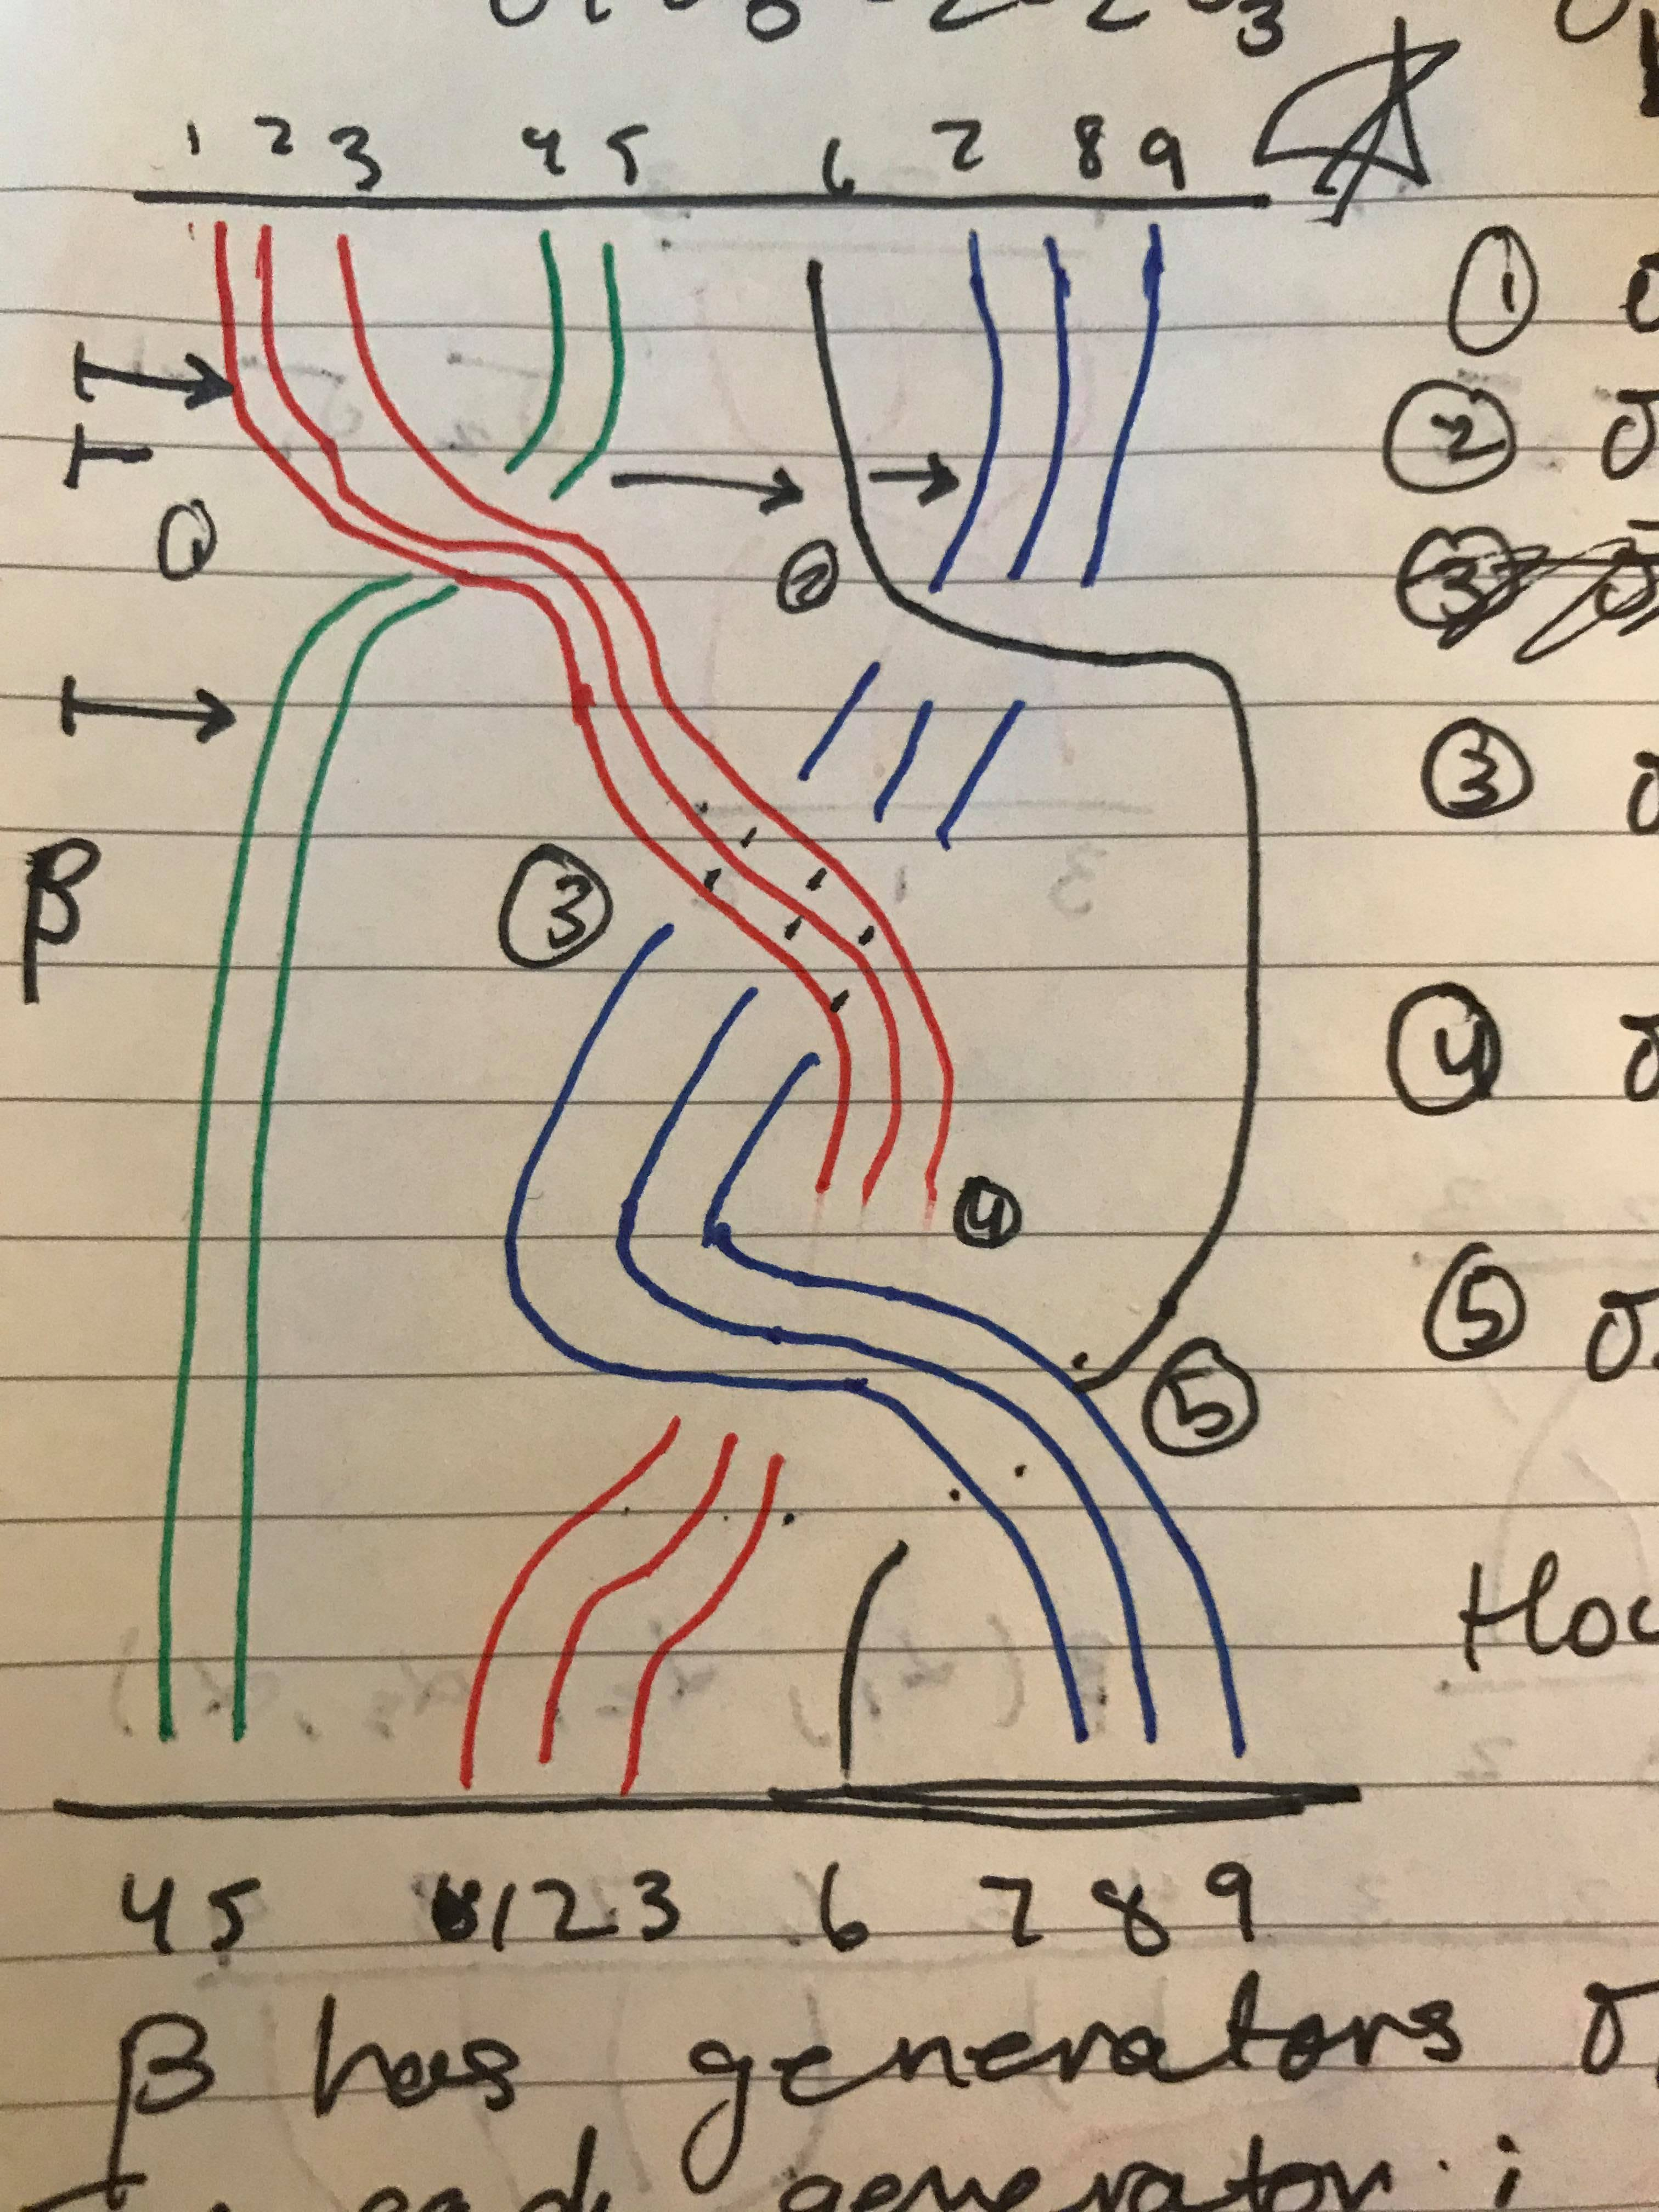
\includegraphics[scale = 0.05]{chp9_operads/braids.jpg}
    
    \emph{Above is the output of $\beta(3, 2, 1, 3)$.}
\end{center}
Staring at the diagram, we can see that it may be expressed as
\begin{gather*}
    (\sigma_3\sigma_2\sigma_1 \cdot \sigma_4\sigma_3\sigma_2) (\sigma_6\sigma_7\sigma_8) 
    (\sigma_5\sigma_4\sigma_3 \cdot \sigma_6\sigma_5\sigma_4 \cdot \sigma_7\sigma_6\sigma_5)\\
    (\sigma_5\sigma_4\sigma_3 \cdot \sigma_6\sigma_5\sigma_4 \cdot \sigma_7\sigma_6\sigma_5)
    (\sigma_8 \sigma_7 \sigma_6).
\end{gather*}
But how can we do this in general? To explain, first suppose 
\[
    \beta = \sigma_{i_1}\sigma_{i_2}\cdots\sigma_{i_k}.
\]
To draw the cabled braid $\beta(k_1, k_2, \dots, k_n)$, we see that we have $k$-crossings to focus on; 
these are where the crossings will happen in our cabled braid. For example, in the braid we provided above, we 
can highlight the crossings in yellow.
\begin{center}
    \def\bottomYCoord{5.5}
\begin{tikzpicture}
    \braid[number of strands= 2, thick,
    style strands={1}{red},
    style strands={2}{Green},
    style strands={3}{Purple},
    style strands={4}{RoyalBlue}]
    (braid) s_1 s_3 s_2 s_2 s_3;
    \filldraw[yellow, opacity = 0.6] (1.5,-0.7) circle (0.3cm);
    \draw (1.5,-0.7) circle (0.3cm);
    \filldraw[yellow, opacity = 0.6] (3.5,-1.7) circle (0.3cm);
    \draw (3.5,-1.7) circle (0.3cm);
    \filldraw[yellow, opacity = 0.6] (2.5,-2.7) circle (0.3cm);
    \draw (2.5,-2.7) circle (0.3cm);
    \filldraw[yellow, opacity = 0.6] (2.5,-3.7) circle (0.3cm);
    \draw (2.5,-3.7) circle (0.3cm);
    \filldraw[yellow, opacity = 0.6] (3.5,-4.7) circle (0.3cm);
    \draw (3.5,-4.7) circle (0.3cm);
    \draw[thick] (0.8,0) -- (4.2,0);
    \draw[thick] (0.8,-\bottomYCoord) -- (4.2,-\bottomYCoord);
\end{tikzpicture}
\end{center}
At each crossing, we're going to have something like this: 
\begin{center}
    \def\bottomYCoord{8.5}
    \begin{tikzpicture}
        \draw[thick] (0.8,0) -- (8.2,0);
        \draw[thick] (0.8,-\bottomYCoord) -- (8.2,-\bottomYCoord);
        \node at (5, -4.2) {
            \begin{tikzpicture}
                \draw[RoyalBlue, thick] plot[smooth,domain=-1.45:1] (\x, {2*\x*\x*\x});
            \end{tikzpicture}
        };
        \node at (5.2, -4.3) {
            \begin{tikzpicture}
                \draw[RoyalBlue, thick] plot[smooth,domain=-1.45:1] (\x, {2*\x*\x*\x});
            \end{tikzpicture}
        };
        \node at (5.5, -4.4) {
            \begin{tikzpicture}
                \draw[RoyalBlue, thick] plot[smooth,domain=-1.35:1.1] (\x, {2*\x*\x*\x});
            \end{tikzpicture}
        };
        %%%%% gaps for braid
        \node at (4.7, -3.9) {
            \begin{tikzpicture}
                \draw[line width = 2mm, white] plot[smooth,domain=-1:1.4] (\x, {-2*\x*\x*\x});
            \end{tikzpicture}
        };
        \node at (4.5, -4) {
            \begin{tikzpicture}
                \draw[line width = 2mm, white] plot[smooth,domain=-1.05:1.4] (\x, {-2*\x*\x*\x});
            \end{tikzpicture}
        };
        \node at (4.1, -4.6) {
            \begin{tikzpicture}
                \draw[line width = 2mm, white] plot[smooth,domain=-1.12:1.32] (\x, {-2*\x*\x*\x});
            \end{tikzpicture}
        };

        %%%%%%% second set of braids
        \node at (4.7, -3.9) {
            \begin{tikzpicture}
                \draw[Red, thick] plot[smooth,domain=-1:1.4] (\x, {-2*\x*\x*\x});
            \end{tikzpicture}
        };
        \node at (4.5, -4) {
            \begin{tikzpicture}
                \draw[Red, thick] plot[smooth,domain=-1.05:1.4] (\x, {-2*\x*\x*\x});
            \end{tikzpicture}
        };
        \node at (4.1, -4.6) {
            \begin{tikzpicture}
                \draw[Red, thick] plot[smooth,domain=-1.12:1.32] (\x, {-2*\x*\x*\x});
            \end{tikzpicture}
        };
        \node at (5,-0.5){
            \begin{tikzpicture}
                \filldraw[white] (0,0) rectangle (9,0.8);
            \end{tikzpicture}
        };
        \node at (5,-8){
            \begin{tikzpicture}
                \filldraw[white] (0,0) rectangle (9,0.8);
            \end{tikzpicture}
        };
        \node at (4, -2.7) {$\vdots$};
        \node at (5.7, -2.7) {$\vdots$};
        \node at (5, -1.7) {$\sigma_{??}$};
    \end{tikzpicture}
\end{center}

That is, at each crossing, there will be a number of red strands crossing over 
blue strands. If we can just describe each of these 
crossings using generators $\sigma_j$ like we did before, 
then we can describe the whole braid. 

We now face the main problem. To describe an arbitrary crossing, we need to know 
which generators $\sigma_1, \sigma_2, \dots, \sigma_{k_1 + \cdots + k_n}$ 
to use, and in general it's not clear which ones to use. For example, 
how do we describe the first crossing? We don't know, so we'll write $\sigma_{??}$. 
If, however, we know that the first red strand is, say the $k$-th strand in $\beta(k_1, \dots, k_n)$,
then we can write the crossing as $\sigma_k$. Then we can travel down the blue line, 
writing $\sigma_{k-1}, \sigma_{k - 2}, \dots$ until we've hit all the red strands. Then 
we can repeat this process for each blue line.

So to do this in general, we need to answer three questions:
\begin{itemize}
    \item How far are all of our red strands from the left? 
    \item How many red strands are there?
    \item How many blue strands are there?
\end{itemize}
If we can answer those three questions, then we can describe exactly what happens 
in terms of generators using formula (\ref{sigma_1_cabling}).

We answer the first question:
\begin{definition}
    Let $\beta \in B_n$ be a braid. Suppose $\beta$ can be written 
    as a product of $k$-many generators $\beta = \sigma_{i_1}\sigma_{i_2} \cdots \sigma_{i_k}$  
    (where any $\sigma$ is equally possibly an inverse). 
    Then we define the quantity 
    \[
        \phi(\sigma_{i_1}\sigma_{i_2}\dots, \sigma_{i_j}, s)
        = 
        \begin{cases}
            \text{The order which strand }s\\
            \text{is from the left after generators}\\
            \sigma_{i_1}\sigma_{i_2}\dots, \sigma_{i_j}
            \text{ have been applied.}
        \end{cases}
    \]
    Of course, $\phi(-, s) = s$, where $-$ represent empty input,
    for each strand $s$. This is because each $s$-th strand is originally the 
    $s$-th strand.

    However, a way to define this is to calculate the underlying permutation 
    of $\sigma_i^{1}\sigma_j^{2}\dots, \sigma_k^{p}$ using the natural projection 
    map $\pi: B_n \to S_n$. Hence we see that 
    \[
        \phi(\sigma_{i_1}\sigma_{i_2}\dots, \sigma_{i_k}, s)
        = 
        \pi(\sigma_{i_1}\sigma_{i_2}\dots, \sigma_{i_k})(s).
    \]
\end{definition}

\begin{example}
    Consider the braid $\sigma_1\sigma_3\sigma_2\sigma_2\sigma_3$ pictured below.
    Suppose we've applied $\sigma_1\sigma_3$. Then our braids are now reordered from how 
    they were initially positioned. For instance, after the application of these 
    generators, the green strand is now the first strand; the red strand is now 
    the second; the blue strand is the third; and the black strand is now the fourth. 
    Each color strand is now in a different position than which it started in.
    \begin{center}
        \def\bottomYCoord{5.5}
        \begin{tikzpicture}
            \braid[number of strands= 2, thick,
            style strands={1}{red},
            style strands={2}{Green},
            style strands={3}{Purple},
            style strands={4}{RoyalBlue}]
            (braid) s_1 s_3 s_2 s_2 s_3;
            \filldraw[yellow, opacity = 0.6] (1.5,-0.7) circle (0.3cm);
            \draw (1.5,-0.7) circle (0.3cm);
            \filldraw[yellow, opacity = 0.6] (3.5,-1.7) circle (0.3cm);
            \draw (3.5,-1.7) circle (0.3cm);
            \draw[thick] (0.8,0) -- (4.2,0);
            \draw[thick] (0.8,-\bottomYCoord) -- (4.2,-\bottomYCoord);
        \end{tikzpicture}
    \end{center}
    However, we can express this observation using our tool.
    Note that $\pi(\sigma_1\sigma_3)$ is the permutation $(1, 2, 3, 4) \mapsto 
    (2, 1, 4, 3)$. Hence we see that 
    \[
        \phi(\sigma_1\sigma_3, 1) = \textcolor{Green}{2} \quad \phi(\sigma_1\sigma_3, 2) = \textcolor{Red}{1} \quad
        \phi(\sigma_1\sigma_3, 3) = \textcolor{RoyalBlue}{4} \quad \phi(\sigma_1\sigma_3, 4) = \textcolor{Purple}{3}.
    \] 
    What about after the first three generators have been applied? We calculate 
    again: $\pi(\sigma_1\sigma_3\sigma_2)$ is the permutation $(1, 2, 3, 4) \mapsto (2, 4, 1, 3)$.
    Hence we have that 
    \[
        \phi(\sigma_1\sigma_3\sigma_2, 1) = \textcolor{Green}{2} \quad \phi(\sigma_1\sigma_3\sigma_2, 2) = \textcolor{NavyBlue}{4} \quad
        \phi(\sigma_1\sigma_3\sigma_2, 3) = \textcolor{red}{1} \quad \phi(\sigma_1\sigma_3\sigma_2, 4) = \textcolor{Purple}{3}.
    \]
    which matches a simple hand-count that we can perform using the picture below.
    \begin{center}
        \begin{tikzpicture}
            \def\bottomYCoord{5.5}
            \braid[number of strands= 2, thick,
            style strands={1}{red},
            style strands={2}{Green},
            style strands={3}{Purple},
            style strands={4}{RoyalBlue}]
            (braid) s_1 s_3 s_2 s_2 s_3;
            \filldraw[yellow, opacity = 0.6] (1.5,-0.7) circle (0.3cm);
            \draw (1.5,-0.7) circle (0.3cm);
            \filldraw[yellow, opacity = 0.6] (3.5,-1.7) circle (0.3cm);
            \draw (3.5,-1.7) circle (0.3cm);
            \filldraw[yellow, opacity = 0.6] (2.5,-2.7) circle (0.3cm);
            \draw (2.5,-2.7) circle (0.3cm);
            \draw[thick] (0.8,0) -- (4.2,0);
            \draw[thick] (0.8,-\bottomYCoord) -- (4.2,-\bottomYCoord);
        \end{tikzpicture}
    \end{center}
\end{example}

This tool allows us to answer our second and third questions. For example, consider again 
$\beta(3, 2, 1, 3)$ where $\beta = \sigma_1\sigma_3\sigma_2\sigma_2\sigma_3$. 
How do we calculate, 
for example, the crossing \raisebox{-0.1cm}{$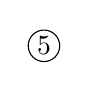
\begin{tikzpicture}\draw (0,0.2) circle(0.2cm) node {5};\end{tikzpicture}$},
of 3 blue lines over 1 black line, as in the picture below?

\begin{center}
    \begin{tikzpicture}
        \braid[number of strands= 2, thick,
        style strands={1}{red},
        style strands={2}{Green},
        style strands={3}{Black},
        style strands={4}{RoyalBlue}]
        (braid) s_1 s_3 s_2 s_2 s_3;
    \end{tikzpicture}
    \hspace{1cm}
    \raisebox{2cm}{$\mapsto$}
    \hspace{1cm}
    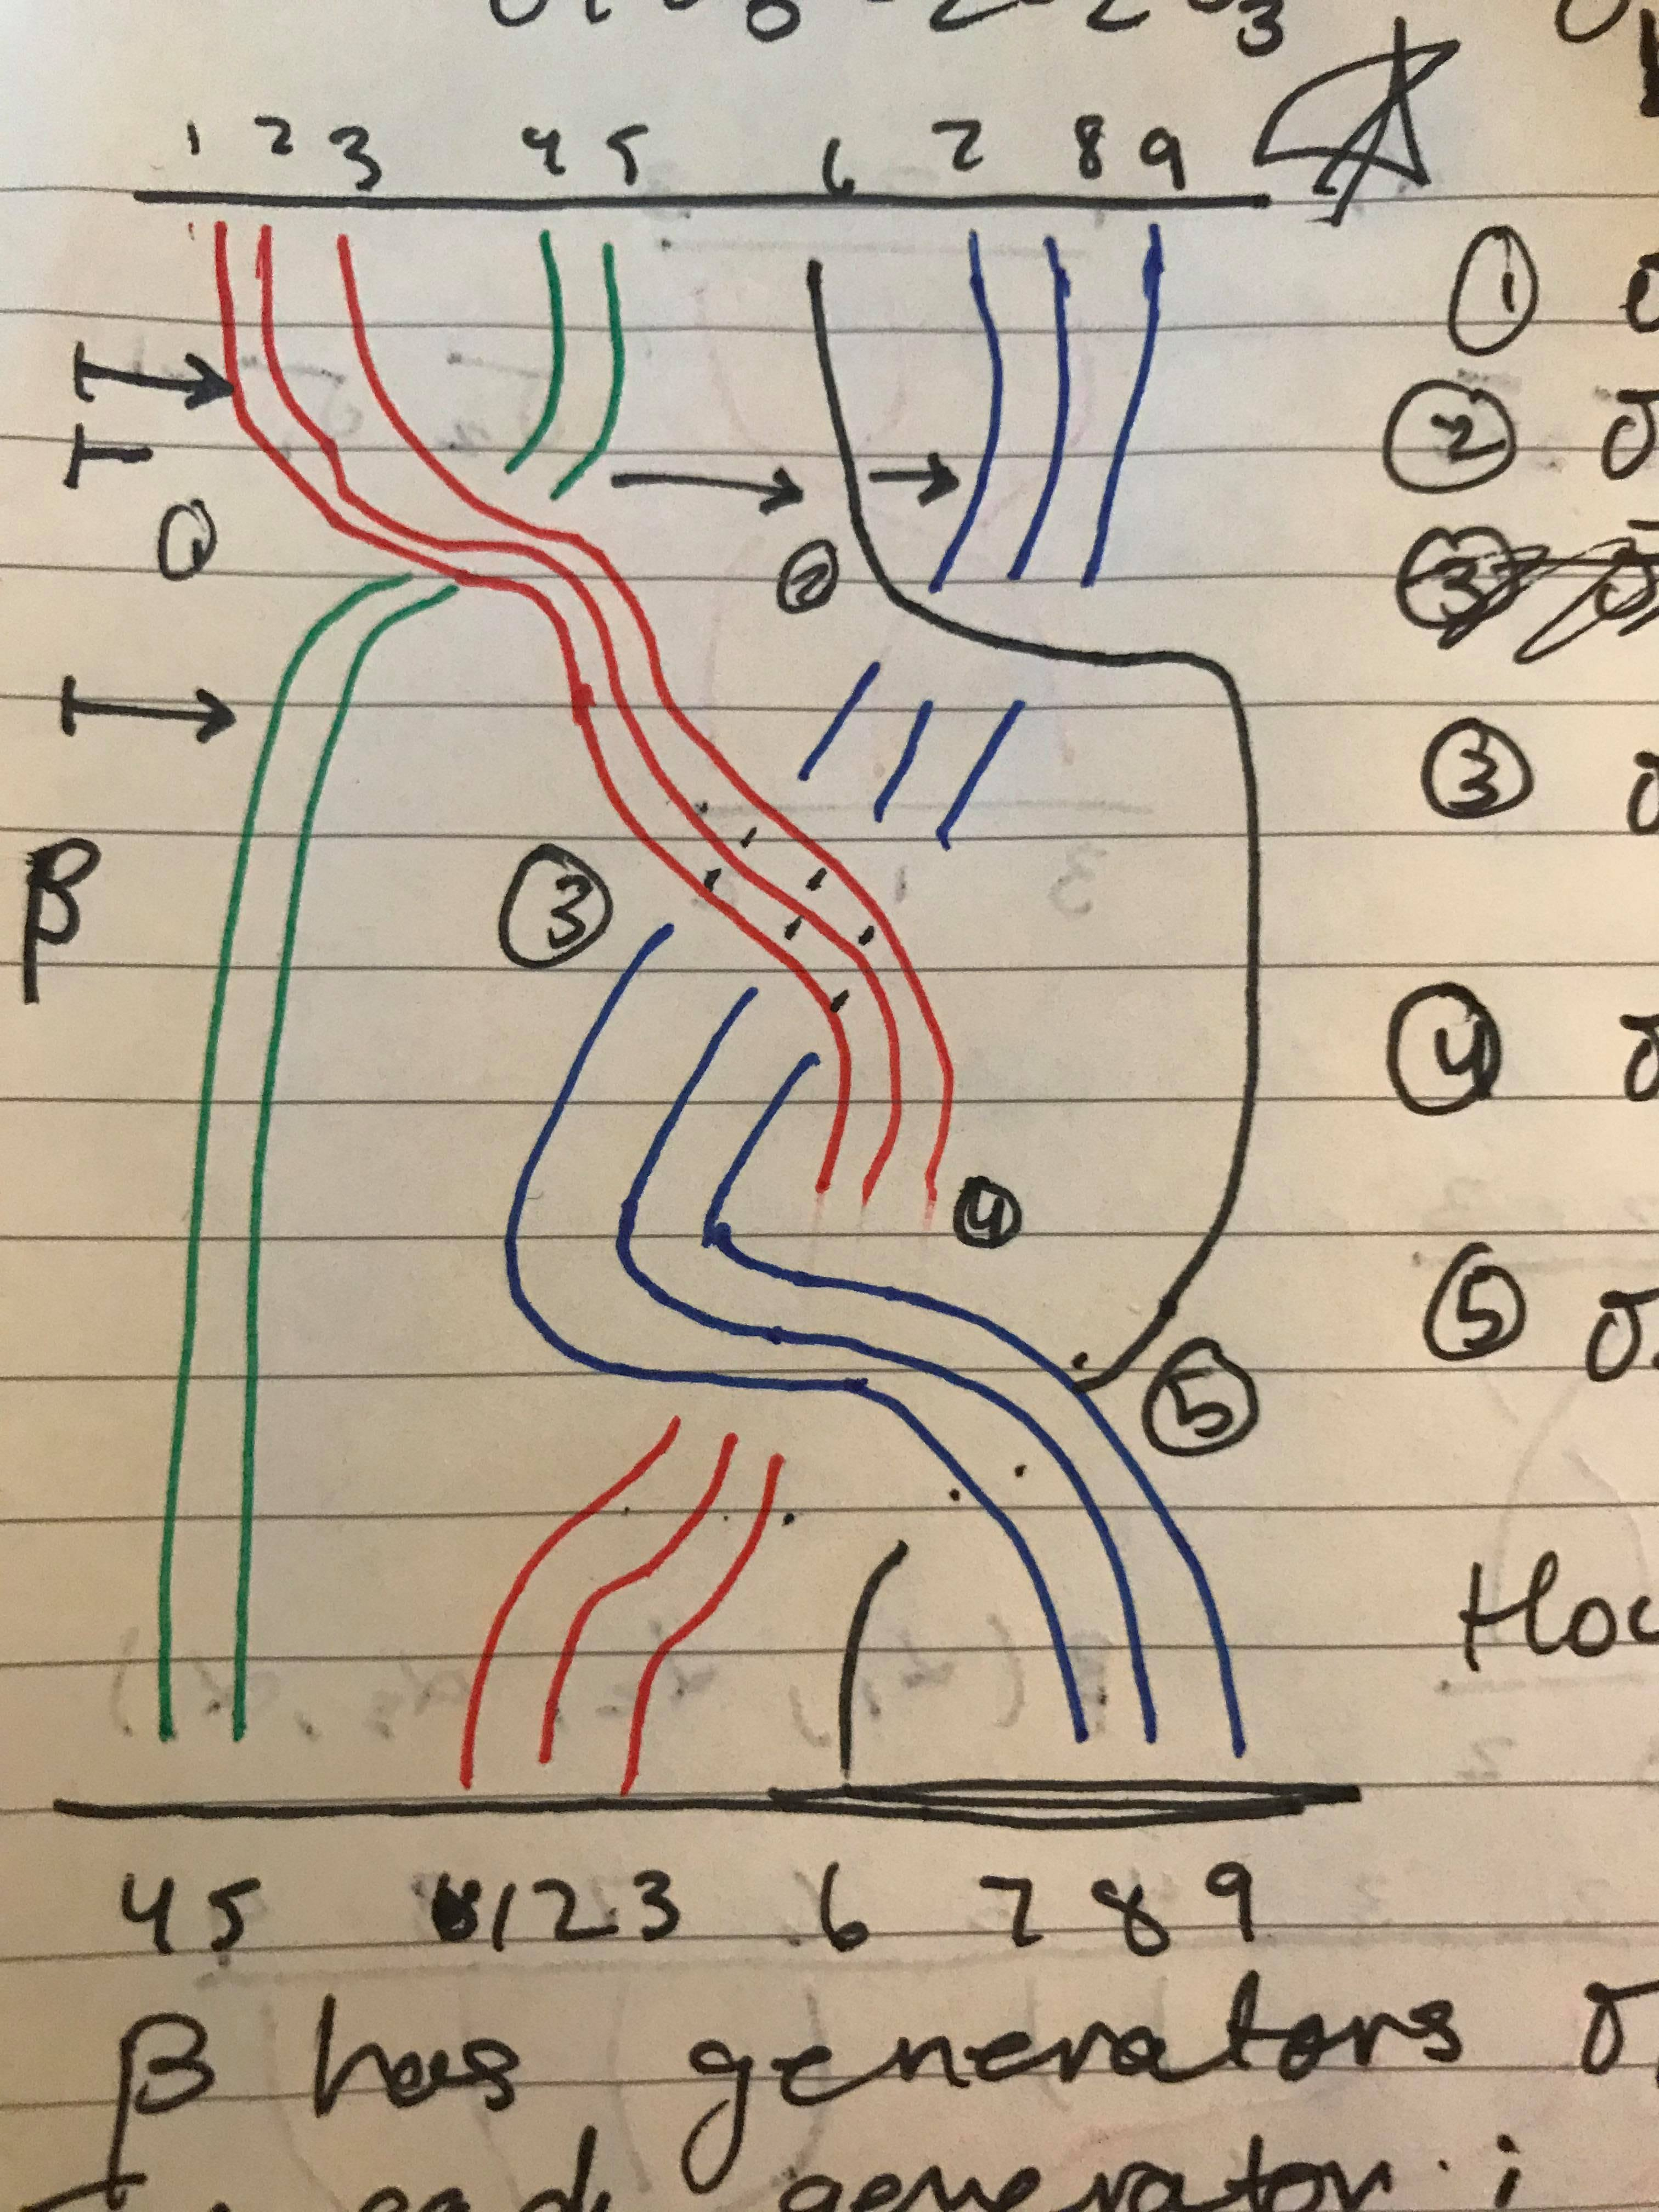
\includegraphics[scale = 0.05]{chp9_operads/braids.jpg}
    
    \emph{Above is the output of $\beta(3, 2, 1, 3)$.}
\end{center}
This crossing is induced by $\sigma_3$, the fifth generator of $\beta$. 
Hence $\beta$ tells us to cross the $3$nd cable over the $4$rd cable. But what 
are these cables? From looking at the diagram, we definitely know. But in general we won't 
be able to just look at the diagram. However, our tool can tell us: Since we've applied $\sigma_1\sigma_3\sigma_2\sigma_2$, 
we see that 
\[
    \phi(\sigma_1\sigma_3\sigma_2\sigma_2, 3) = \textcolor{RoyalBlue}{4} \qquad \phi(\sigma_1\sigma_3\sigma_2\sigma_2, 4) = \textcolor{Black}{1}.
\]
Therefore, we're crossing blue cables over the black cables. We also now know there
are $k_{\textcolor{RoyalBlue}{4}} = 3$ blue cables and $k_{\textcolor{Black}{3}} = 1$ many black cables.
We have almost everything we need except the following: how far 
are the blue cables from the left of the diagram? 

Well, since the blue strands are inside of the third cable, we just need to ask how many 
stands are in the first and second cables. But what is the first cable? What's the second?
We see that
\[
    \phi(\sigma_1\sigma_3\sigma_2\sigma_2, 1) =  \textcolor{Green}{2}.
    \quad 
    \phi(\sigma_1\sigma_3\sigma_2\sigma_2, 2) = \textcolor{Red}{1}.
\]
Hence there are 
\[
    k_{\textcolor{Green}{2}} + k_{\textcolor{Red}{1}} = 2 + 3 = 5    
\]
strands before the blue strands. We can now calculate the crossings: 
\begin{align*}
    \sigma_{5 + 3}\sigma_{5 + 2} \sigma_{5 + 1}
    &=
    \prod_{m = 1 + 5}^{1 + 5}\sigma_{3 + (m - 1)}\sigma_{3 + (m - 2)}\sigma_m\\
    &=
    \prod_{m = p}^{p + (r - 1)}\sigma_{q + (m - 1)}\sigma_{q + (m - 2)}\sigma_m
\end{align*}
where 
\[
    p = 1 + \hspace{-1.5cm}\overbrace{k_2 + k_3}^{\text{\# of strands before the red strands}}
    \quad 
    q = \hspace{-1cm}\underbrace{k_{\textcolor{RoyalBlue}{4}}}_{\text{\# of strands in the 3rd cable}}
    r = \hspace{-1cm}\overbrace{k_{\textcolor{Black}{3}}}^{\text{\# of strands in the 4th cable}}
\]


Therefore we propose the following. 
\begin{lemma}
    Let $\beta \in B_n$ be a braid, and suppose it 
    may be expressed as $\sigma_{i_1}\sigma_{i_2} \cdots \sigma_{i_k}$ in terms of $k$-many 
    generators. Let $k_1, \dots, k_n$ be positive integers. Then we have that 
    \[
        \beta(k_1, k_2, \dots, k_n) 
        = 
        \psi_1\psi_2\dots\psi_k
    \]  
    where, depending on if $\sigma_{i_j}$ is an instance of an inverse or not, 
    we have 
    \begin{statement}{ProcessBlue!10}
    \[
        \prod_{m = p_j}^{p_j + (r_j-1)}
        \sigma_{q_j + (m-1)}
        \sigma_{q_j + (m-2)}
        \cdots 
        \sigma_{m}
        \quad 
        \text{ or }
        \quad 
        \prod_{m = p_j}^{p_j + (r_j-1)}
        \sigma^{-1}_{(q_j + m) - 1}
        \sigma^{-1}_{(q_j -m) - 2}
        \cdots 
        \sigma^{-1}_{m}
    \]
    \end{statement}
    where in both cases
    \begin{statement}{ProcessBlue!10}
    \[
        p_j
        =
        \overbrace{
        1 +
        \sum_{u = 1}^{i_j-1}
        k_{\phi(\sigma_{i_1}\cdots\sigma_{i_{j-1}}, u)}
        }^{\text{\# strands before } i_j\text{-th cable} }
        \qquad
        \underbrace{
        q_j = 
        k_{\phi(\sigma_{i_1}\cdots\sigma_{i_{j-1}}, i_j)}
        }_{\text{\# of strands in the }i_j \text{-th cable}}
        \qquad 
        \overbrace{
        r_j
        =
        k_{\phi(\sigma_{i_1}\cdots\sigma_{i_{(j-1)}}, (i_j+1))}
        }^{\text{\# of stands in the } (i_j+1)\text{-th cable} }
    \]
    \end{statement}
\end{lemma}

The three quantities are the three answers to our original questions: 
\begin{itemize}
    \item After applying $\sigma_{i_1}\dots\sigma_{i_{j-1}}$,
    how many strands come before the cable $i_j$, relative to the left? $p_j$.
    \item 
    How many strands are in the $i_j$-th cable after applying $\sigma_{i_1}\dots\sigma_{i_{j-1}}$? 
    $q_j$.
    \item How many strands are in the $(i_j+1)$-th after applying $\sigma_{i_1}\dots\sigma_{i_{j-1}}$? 
    $r_j$.
\end{itemize}

\begin{example}
    We can apply this to our previous example. 
    Recall that $\beta = \sigma_1\sigma_3\sigma_2\sigma_2\sigma_3$. 
    One way to interpret out braid diagram is as a sequence of permutations.
    In this case we see that we get five permutations because we have five generators.
    \begin{center}
        \def\bottomYCoord{5.5}
        \begin{tikzpicture}
            \braid[number of strands= 2, thick,
            style strands={1}{red},
            style strands={2}{Green},
            style strands={3}{Purple},
            style strands={4}{RoyalBlue}]
            (braid) s_1 s_3 s_2 s_2 s_3;
            % \filldraw[yellow, opacity = 0.6] (1.5,-0.7) circle (0.3cm);
            % \draw (1.5,-0.7) circle (0.3cm);
            % \filldraw[yellow, opacity = 0.6] (3.5,-1.7) circle (0.3cm);
            % \draw (3.5,-1.7) circle (0.3cm);
            \draw[thick] (0.8,0) -- (4.2,0);
            \draw[thick] (0.8,-\bottomYCoord) -- (4.2,-\bottomYCoord);
            \node at (1, -5.7) {\phantom{2}};
            \node at (2, -5.7) {\phantom{1}};
            \node at (3, -5.7) {\phantom{4}};
            \node at (4, -5.7) {\phantom{3}};
        \end{tikzpicture}
        \raisebox{3cm}{$\mapsto$}
        \begin{tikzpicture}
            \braid[number of strands= 2, thick,
            style strands={1}{red},
            style strands={2}{Green},
            style strands={3}{Purple},
            style strands={4}{RoyalBlue}]
            (braid) s_1 s_3 s_2 s_2 s_3;
            % \filldraw[yellow, opacity = 0.6] (1.5,-0.7) circle (0.3cm);
            % \draw (1.5,-0.7) circle (0.3cm);
            % \filldraw[yellow, opacity = 0.6] (3.5,-1.7) circle (0.3cm);
            % \draw (3.5,-1.7) circle (0.3cm);
            \draw[thick] (0.8,0) -- (4.2,0);
            \draw (0.8,-1.4) -- (4.2,-1.4); %first bar
            \draw (0.8,-2.3) -- (4.2,-2.3); %second bar
            \draw (0.8,-3.3) -- (4.2,-3.3); %third bar
            \draw (0.8,-4.3) -- (4.2,-4.3); %fourth bar
            
            %first set
            \node at (1, 0.2) {1};
            \node at (2, 0.2) {2};
            \node at (3, 0.2) {3};
            \node at (4, 0.2) {4};
            %second set
            \node at (1.2, -1.2) {2};
            \node at (2.2, -1.2) {1};
            \node at (3.2, -1.2) {3};
            \node at (4.2, -1.2) {4};
            %third set 
            \node at (1.2, -2.1) {2};
            \node at (2.2, -2.1) {1};
            \node at (3.2, -2.1) {4};
            \node at (4.2, -2.1) {3};
            %fourth set 
            \node at (1.2, -3.1) {2};
            \node at (2.2, -3.1) {4};
            \node at (3.2, -3.1) {1};
            \node at (4.2, -3.1) {3};
            %fifth set 
            \node at (1.2, -4.1) {2};
            \node at (2.2, -4.1) {1};
            \node at (3.2, -4.1) {4};
            \node at (4.2, -4.1) {3};
            %sixth set 
            \node at (1, -5.7) {2};
            \node at (2, -5.7) {1};
            \node at (3, -5.7) {3};
            \node at (4, -5.7) {4};
            \draw[thick] (0.8,-\bottomYCoord) -- (4.2,-\bottomYCoord);
        \end{tikzpicture}
    \end{center}

    First we compute the table 
    \begin{center}
        \begin{tabular}{|c|c |c| c| c|} 
            \hline
            $j$ & $i_{j}$ & $p_j$ & $q_j$ & $r_j$ \\ [0.5ex] 
            \hline
            1 & 1 & 1 &$k_1 = 3$ & $k_2 = 2$ \\ 
            \hline
            2 & 3 & $1 + k_1 + k_2 = 6$ & $k_3 = 1$ & $k_4 = 3$ \\
            \hline
            3 & 2 & $1 + k_2 = 3$ & $k_1 = 3$ & $k_4 = 3$ \\
            \hline
            4 & 2 & $1 + k_2 = 3$ & $k_4 = 3$ & $k_1 = 3$ \\
            \hline
            5 & 3 & $1 + k_1 + k_2 = 6$ & $k_4 = 3$ & $k_3 = 1$ \\ [1ex] 
            \hline
           \end{tabular}
    \end{center}
    This then gives us the product 
    \begin{gather*}
        \left(\prod_{m = p_1}^{p_1 + (r_1-1)}
        \sigma_{q_1 + (m-1)}
        \sigma_{q_1 + (m-2)}
        \cdots 
        \sigma_{m}\right)
        \left(\prod_{m = p_2}^{p_2 + (r_2-1)}
        \sigma_{q_2 + (m-1)}
        \sigma_{q_2 + (m-2)}
        \cdots 
        \sigma_{m} \right)
        \\
        \left(     \prod_{m = p_3}^{p_3 + (r_3-1)}
        \sigma_{q_3 + (m-1)}
        \sigma_{q_3 + (m-2)}
        \cdots 
        \sigma_{m} \right)
        \\
        \left(    \prod_{m = p_4}^{p_4 + (r_4-1)}
        \sigma_{q_4 + (m-1)}
        \sigma_{q_4 + (m-2)}
        \cdots 
        \sigma_{m} \right)
        \left(     \prod_{m = p_5}^{p_5 + (r_5-1)}
        \sigma_{q_5 + (m-1)}
        \sigma_{q_5 + (m-2)}
        \cdots 
        \sigma_{m} \right)
    \end{gather*}
    which becomes 
    \begin{gather*}
        \left(\prod_{m = 1}^{1 + (2-1)}
        \sigma_{3 + (m-1)}
        \sigma_{3 + (m-2)}
        \cdots 
        \sigma_{m}\right)
        \left(\prod_{m = 6}^{6 + (3-1)}
        \sigma_{1 + (m-1)}
        \sigma_{1 + (m-2)}
        \cdots 
        \sigma_{m} \right)
        \\
        \left(     \prod_{m = 3}^{3 + (3-1)}
        \sigma_{3 + (m-1)}
        \sigma_{3 + (m-2)}
        \cdots 
        \sigma_{m} \right)
        \\
        \left(    \prod_{m = 3}^{3 + (3-1)}
        \sigma_{3 + (m-1)}
        \sigma_{3 + (m-2)}
        \cdots 
        \sigma_{m} \right)
        \left(     \prod_{m = 6}^{6 + (1-1)}
        \sigma_{3 + (m-1)}
        \sigma_{3 + (m-2)}
        \cdots 
        \sigma_{m} \right)
    \end{gather*}
    which reduces to 
    \begin{gather*}
        (\sigma_3\sigma_2\sigma_1 \cdot \sigma_4\sigma_3\sigma_2)
        (\sigma_6 \sigma_7\sigma_8)(\sigma_5\sigma_4\sigma_3\cdot \sigma_6\sigma_5\sigma_4 \cdot \sigma_7\sigma_6\sigma_5)
        \\
        (\sigma_5\sigma_4\sigma_3\cdot \sigma_6\sigma_5\sigma_4 \cdot \sigma_7\sigma_6\sigma_5)
        (\sigma_8\sigma_7\sigma_6)
    \end{gather*}
    which correctly matches what we had before. 
\end{example}

\begin{example}
    We haven't looked at a braid with an under crossing. So, 
    consider the braid $\beta = \sigma_1^{-1}\sigma_2^{-1}\sigma_3\sigma_2\sigma_1 \in B_4$, 
    and let $k_1 = 2, k_2 = 3, k_3 = 4, k_4 = 5$. We'll want to calculate 
    the braid $\beta(2, 3, 4, 5)$. Below is $\beta$ and $\beta(2,3,4,5)$.
    \begin{center}
    \def\bottomYCoord{5.5}
    \begin{tikzpicture}
        \braid[number of strands= 4, thick, 
        style strands={1}{Red},
        style strands={2}{Green},
        style strands={3}{Purple},
        style strands={4}{RoyalBlue}]
        (braid) s_1^{-1} s_2^{-1} s_3 s_2 s_1;
        \draw[thick] (0.8,0) -- (4.2,0);
        \draw[thick] (0.8,-\bottomYCoord) -- (4.2,-\bottomYCoord);
    \end{tikzpicture}
    \hspace{1cm}
    \raisebox{2cm}{$\mapsto$}
    \hspace{1cm}
    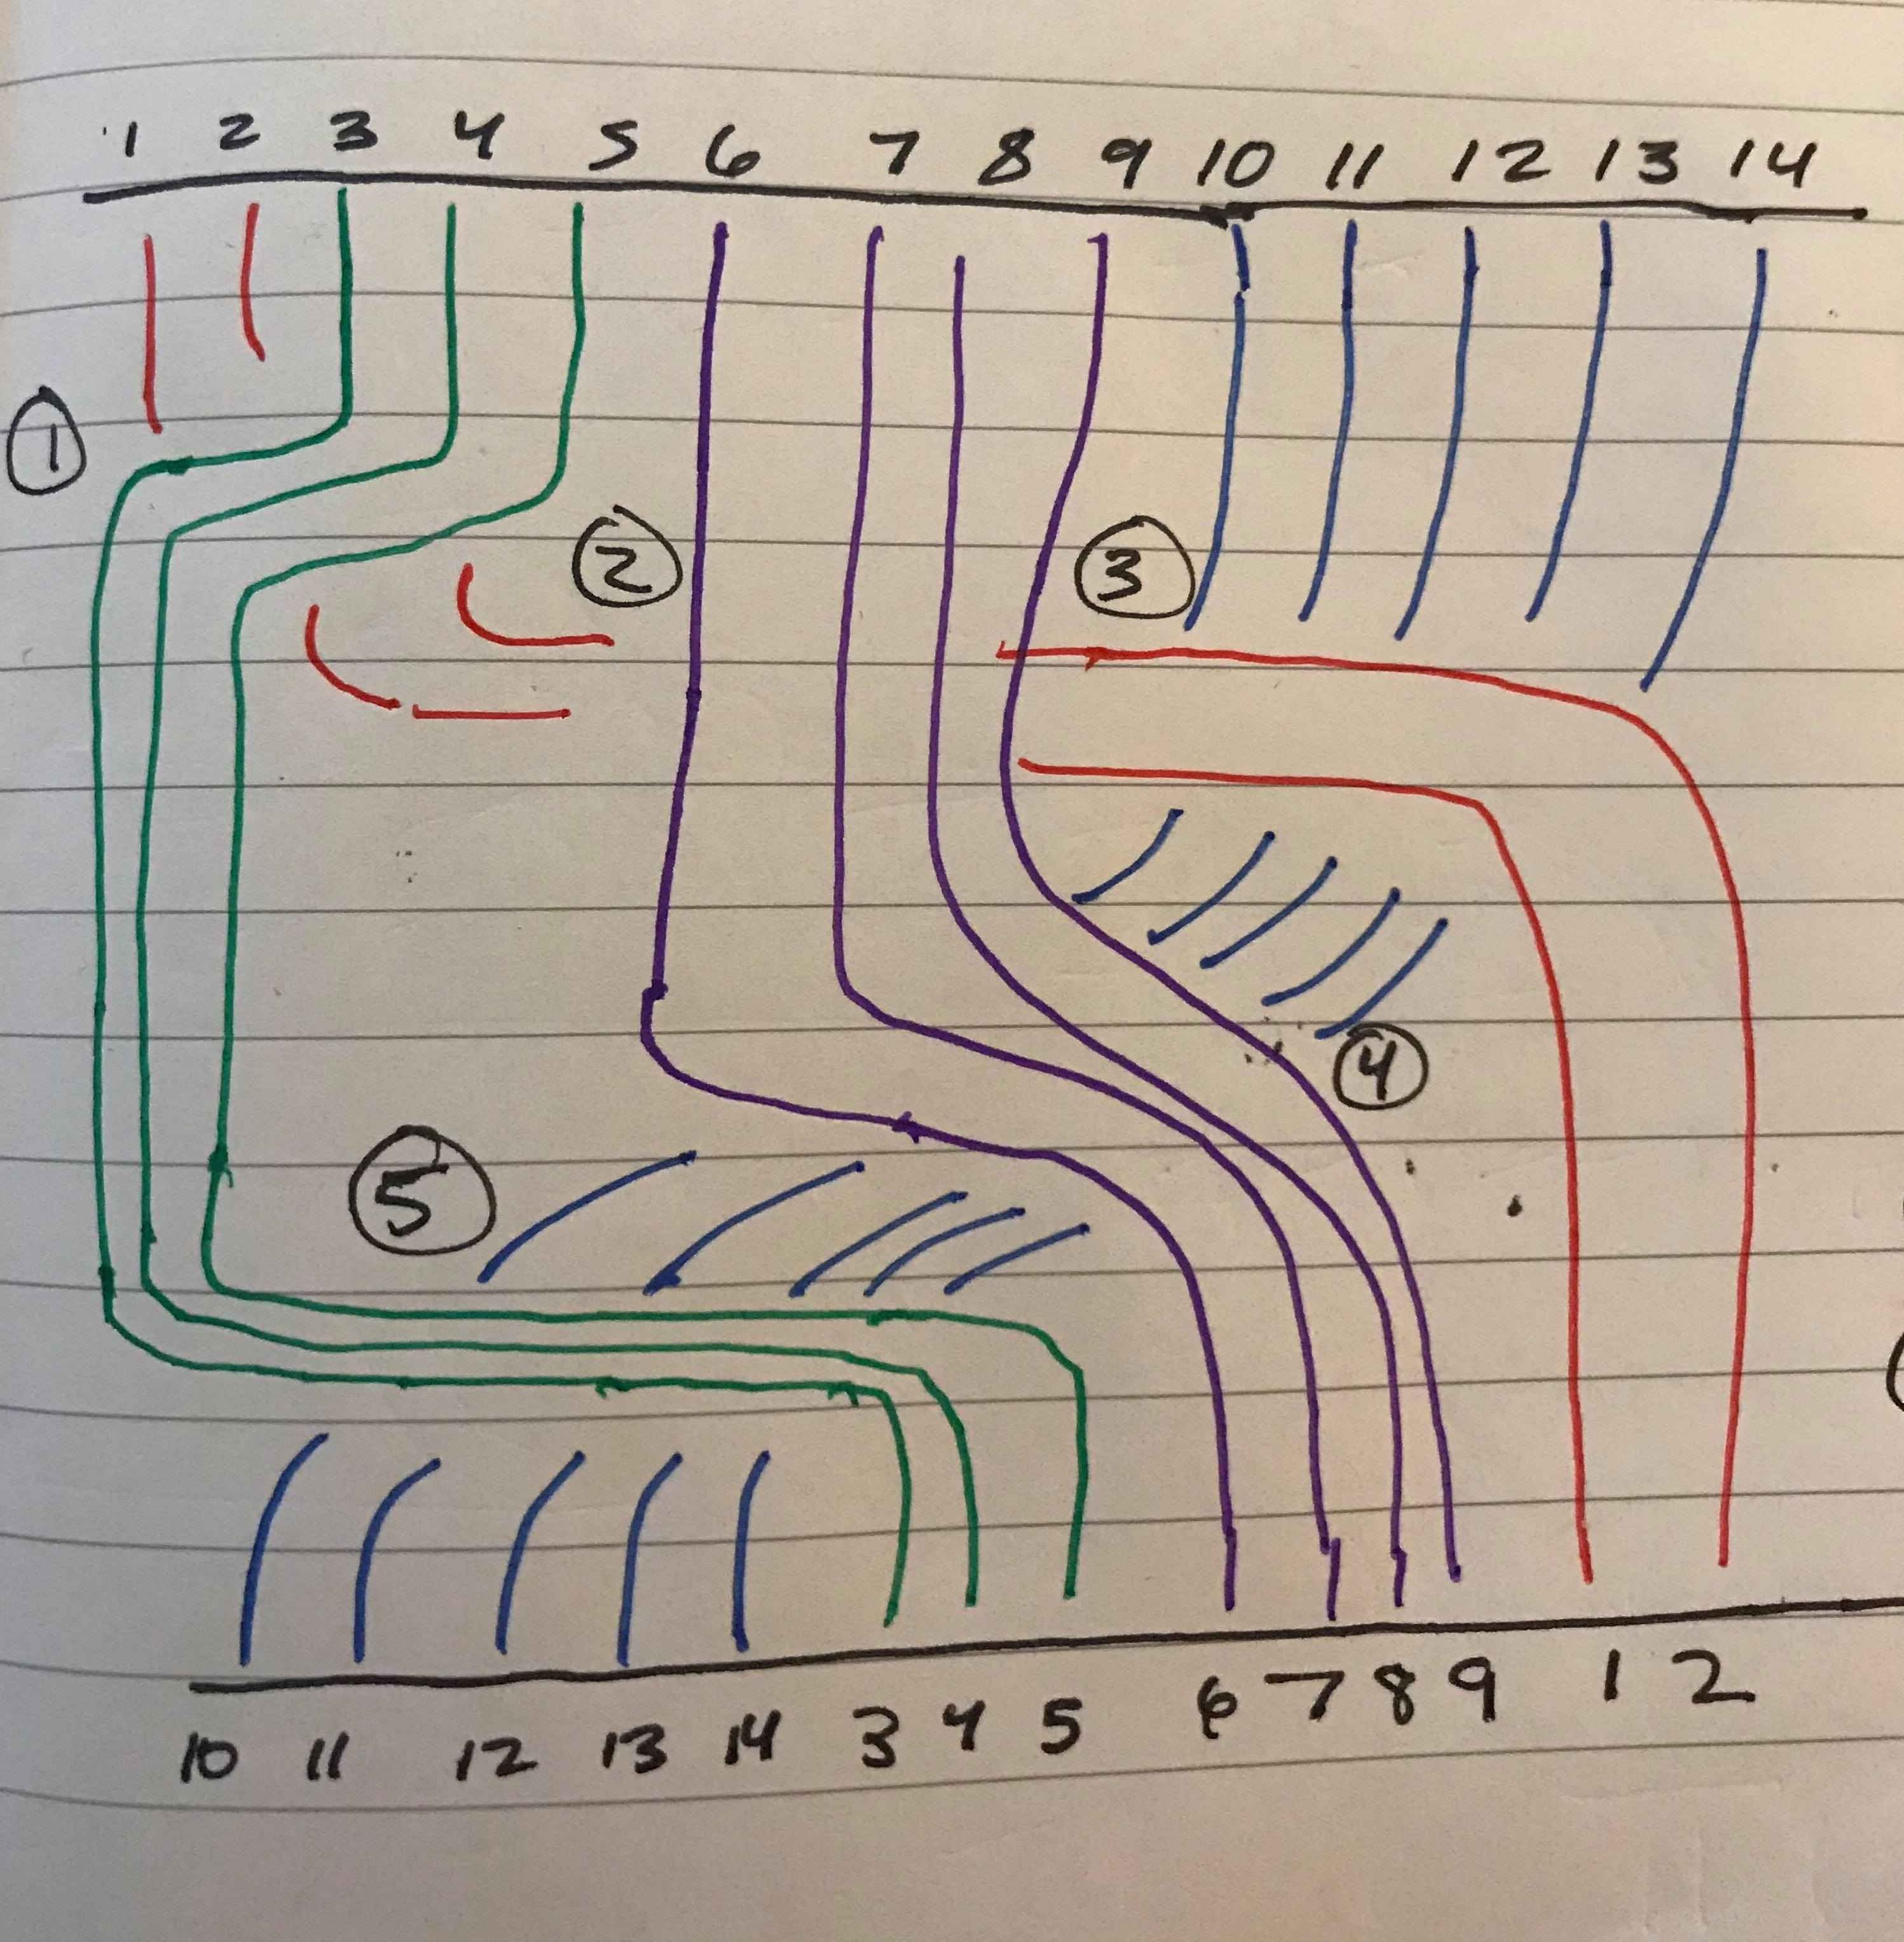
\includegraphics[scale = 0.06]{chp9_operads/inverse_braids.jpg}
    \end{center}
    To calculate the resulting braid we need to create our table of values.
    This is more easily done by generating the permutation table on the left; it 
    tells us how our cables are swapped around. 
    \begin{center}
        \begin{tabular}{|l|c|}
            \hline
            Generator & Permutation\\
            \hline
            $\varnothing$ & $(\textcolor{Red}{1}, \textcolor{Green}{2}, \textcolor{Purple}{3}, \textcolor{RoyalBlue}{4})$\\
            \hline
            $\sigma_1^{-1}$ & $(\textcolor{Green}{2}, \textcolor{Red}{1}, \textcolor{Purple}{3}, \textcolor{RoyalBlue}{4})$\\
            \hline
            $\sigma_1^{-1}\sigma_2^{-1}$ & $(\textcolor{Green}{2}, \textcolor{Purple}{3}, 1, \textcolor{RoyalBlue}{4})$\\
            \hline
            $\sigma_1^{-1}\sigma_2^{-1}\sigma_3$ & $(\textcolor{Green}{2}, \textcolor{Purple}{3}, \textcolor{RoyalBlue}{4}, 1)$\\
            \hline
            $\sigma_1^{-1}\sigma_2^{-1}\sigma_3\sigma_2$ & $(\textcolor{Green}{2}, \textcolor{RoyalBlue}{4}, \textcolor{Purple}{3}, 1)$\\
            \hline
            $\sigma_1^{-1}\sigma_2^{-1}\sigma_3\sigma_2\sigma_1$ & $(\textcolor{RoyalBlue}{4}, \textcolor{Green}{2}, \textcolor{Purple}{3}, 1)$\\
            \hline
        \end{tabular}
        \hspace{1cm}
        \begin{tabular}{|c|c |c| c| c|} 
            \hline
            $j$ & $i_{j}$ & $p_j$ & $q_j$ & $r_j$ \\ [1ex] 
            \hline
            1 & 1 & 1 & $k_1 = 2$  & $k_2 = 3$  \\ [.1ex] 
            \hline
            2 & 2 & $1 + k_2 = 4$ & $k_1 =2$ & $k_3 = 4$ \\ [.1ex] 
            \hline
            3 & 3 & $1 + k_2 + k_3 = 8$ & $k_1 = 2$ & $k_4 = 5$ \\ [.1ex] 
            \hline
            4 & 2 & $1 + k_2 = 4$ & $k_3 =4$ & $k_4 = 5$ \\[.1ex] 
            \hline
            5 & 1 & $1$ & $k_2 = 3$ & $k_4 = 5$\\ [1ex] 
            \hline
           \end{tabular}
    \end{center}
    This then generates the products 
    \begin{gather*}
        \left(\prod_{m = 1}^{3}\sigma_{m + 2}^{-1}\sigma^{-1}_m\right)
        \left( \prod_{m = 4}^{7}\sigma^{-1}_{(m+2)-1}\sigma_m^{-1} \right)
        \left( \prod_{m = 8}^{12}\sigma_{(m+2)-1}\sigma_m \right)
        \left( \prod_{m = 4}^{8}\sigma_{(m+4)-1}\sigma_{(m+4)-2}\sigma_{(m+4)-3}\sigma_{m} \right)
        \\
        \left( \prod_{m = 1}^{5}\sigma_{(m+3)-1}\sigma_{(m+3)-2}\sigma_m \right)
    \end{gather*}
    which becomes 
    \begin{gather*}
        (\sigma^{-1}_2\sigma^{-1}_1 \cdot \sigma^{-1}_3\sigma^{-1}_2 \cdot \sigma^{-1}_4\sigma^{-1}_3)
        (\sigma^{-1}_5\sigma^{-1}_4\cdot \sigma^{-1}_6\sigma^{-1}_5 \cdot \sigma^{-1}_7\sigma^{-1}_6 \cdot \sigma^{-1}_8\sigma^{-1}_7)
        \\
        (\sigma_9\sigma_8 \cdot \sigma_{10}\sigma_9 \cdot \sigma_{11}\sigma_{10} \cdot \sigma_{12}\sigma_{11} \cdot \sigma_{13}\sigma_{12})
        (\sigma_7\sigma_6\sigma_5\sigma_4 \cdot \sigma_8\sigma_7\sigma_6\sigma_5 \cdot \sigma_9\sigma_8\sigma_7\sigma_6 \cdot 
        \sigma_{10}\sigma_9\sigma_8\sigma_7\cdot \sigma_{11}\sigma_{10}\sigma_9\sigma_8)
        \\
        (\sigma_3\sigma_2\sigma_1 \cdot \sigma_4\sigma_3\sigma_2 \cdot \sigma_5\sigma_4\sigma_3 \cdot \sigma_6\sigma_5\sigma_4 \cdot \sigma_7\sigma_6\sigma_5)
    \end{gather*}
    which is the correct description of the braid $\beta(2,3,4,5)$. 
\end{example}

Now we can finally answer our desired question: 
\begin{center}
    Given a braid $\beta \in B_n$, and $n$ other braids $\alpha_1 \in B_{a_1}, \dots, \alpha_n \in B_{a_n}$, 
    what is the formula for $\beta(\alpha_1, \dots, \alpha_n)$? 
\end{center}

To answer this question, we build on our previous work by making the following observation. 
Suppose we want to compute $\sigma_1(\alpha_1, \alpha_2)$ where $\sigma_1, \alpha_1, \alpha_2$
appear as below.
\begin{center}
    \def\bottomYCoord{3.5}
    \begin{tikzpicture}
        \braid[number of strands= 2, thick,  height = 3cm]
        s_1;
        \draw[thick] (0.8,0) -- (2.2,0);
        \draw[thick] (0.8,-\bottomYCoord) -- (2.2,-\bottomYCoord);
    \end{tikzpicture}
    \hspace{1cm}
    \begin{tikzpicture}
        \braid[number of strands= 3, thick, 
        style strands={1}{Green},
        style strands={2}{Green},
        style strands={3}{Green}]
        s_2 s_1 s_2;
        \draw[thick] (0.8,0) -- (3.2,0);
        \draw[thick] (0.8,-\bottomYCoord) -- (3.2,-\bottomYCoord);
    \end{tikzpicture}
    \hspace{1cm}
    \begin{tikzpicture}
        \braid[number of strands= 3, thick, height = 1.5cm,
        style strands={1}{Red},
        style strands={2}{Red},
        style strands={3}{Red}]
        s_2 s_1;
        \draw[thick] (0.8,0) -- (3.2,0);
        \draw[thick] (0.8,-\bottomYCoord) -- (3.2,-\bottomYCoord);
    \end{tikzpicture}

    \emph{Here we have $\sigma_1$, $\alpha_1= \sigma_2\sigma_1\sigma_2$ 
    and $\alpha_2 = \sigma_2\sigma_1$.}
\end{center}

Then we get the braid diagram as in \raisebox{-0.1cm}{$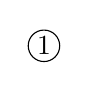
\begin{tikzpicture}\draw (0,0.2) circle(0.2cm) node {1};\end{tikzpicture}$}.
\begin{center}
    \includegraphics[scale = 0.1]{braids_cabled.jpg}
\end{center}
However, we can all isotopies to stretch the braid to \raisebox{-0.1cm}{$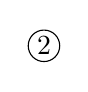
\begin{tikzpicture}\draw (0,0.2) circle(0.2cm) node {2};\end{tikzpicture}$}, 
then \raisebox{-0.1cm}{$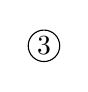
\begin{tikzpicture}\draw (0,0.2) circle(0.2cm) node {3};\end{tikzpicture}$}, 
and then reaching a final stage of \raisebox{-0.1cm}{$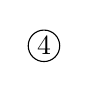
\begin{tikzpicture}\draw (0,0.2) circle(0.2cm) node {4};\end{tikzpicture}$}. 
But note that \raisebox{-0.1cm}{$\begin{tikzpicture}\draw (0,0.2) circle(0.2cm) node {4};\end{tikzpicture}$}
may be expressed in either of the equivalent ways:
\\

\begin{minipage}{0.5\textwidth}
    \begin{center}
        \def\bottomYCoord{9.5}
        \begin{tikzpicture}
            \braid[number of strands= 6, thick, 
            style strands={1}{Green},
            style strands={2}{Green},
            style strands={3}{Green},
            style strands={4}{Red},
            style strands={5}{Red},
            style strands={6}{Red},
            gap = 0.1,
            control factor=.001,
            nudge factor=.001,
            ]
            s_3 s_2 s_1 s_4 s_3 s_2 s_5 s_4 s_3;
            \draw[thick] (0.8,0) -- (6.2,0);
            \draw[thick] (0.8,-\bottomYCoord) -- (6.2,-\bottomYCoord);
        \end{tikzpicture}
    \end{center}
    \begin{center}
        \def\bottomYCoord{3.5}
        \begin{tikzpicture}
            \braid[number of strands= 3, thick, height = 1.5cm,
            style strands={1}{Red},
            style strands={2}{Red},
            style strands={3}{Red},
            ]
            s_2 s_1;
            \draw[thick] (0.8,0) -- (3.2,0);
            \draw[thick] (0.8,-\bottomYCoord) -- (3.2,-\bottomYCoord);
        \end{tikzpicture}
        \hspace{0.3cm}
        \begin{tikzpicture}
            \braid[number of strands = 3, thick,
            style strands={1}{Green},
            style strands={2}{Green},
            style strands={3}{Green},
            ]
            s_2 s_1 s_2;
            \draw[thick] (0.8,0) -- (3.2,0);
            \draw[thick] (0.8,-\bottomYCoord) -- (3.2,-\bottomYCoord);
        \end{tikzpicture}
    \end{center}
\end{minipage}
\begin{minipage}{0.5\textwidth}
    \begin{center}
        \def\bottomYCoord{3.5}
        \begin{tikzpicture}
            \braid[number of strands = 3, thick,
            style strands={1}{Green},
            style strands={2}{Green},
            style strands={3}{Green},
            ]
            s_2 s_1 s_2;
            \draw[thick] (0.8,0) -- (3.2,0);
            \draw[thick] (0.8,-\bottomYCoord) -- (3.2,-\bottomYCoord);
        \end{tikzpicture}
        \hspace{0.3cm}
        \begin{tikzpicture}
            \braid[number of strands= 3, thick, height = 1.5cm,
            style strands={1}{Red},
            style strands={2}{Red},
            style strands={3}{Red},
            ]
            s_2 s_1;
            \draw[thick] (0.8,0) -- (3.2,0);
            \draw[thick] (0.8,-\bottomYCoord) -- (3.2,-\bottomYCoord);
        \end{tikzpicture}
    \end{center}
    \begin{center}
        \def\bottomYCoord{9.5}
        \begin{tikzpicture}
            \braid[number of strands= 6, thick, 
            style strands={1}{Green},
            style strands={2}{Green},
            style strands={3}{Green},
            style strands={4}{Red},
            style strands={5}{Red},
            style strands={6}{Red},
            gap = 0.1,
            control factor=.001,
            nudge factor=.001,
            ]
            s_3 s_2 s_1 s_4 s_3 s_2 s_5 s_4 s_3;
            \draw[thick] (0.8,0) -- (6.2,0);
            \draw[thick] (0.8,-\bottomYCoord) -- (6.2,-\bottomYCoord);
        \end{tikzpicture}
    \end{center}
\end{minipage}
\vspace{1cm}

This then gives us the following idea. Suppose we want to calculate 
$\beta(\alpha_1, \dots, \alpha_n)$ where $\alpha_i \in B_{a_i}$.
Define $\alpha_1\oplus \dots \oplus \alpha_n$ as the $(a_1 + \cdots + a_n)$-braid. 
Suppose that $\alpha_j = \sigma_{j, i_j}, \dots, \sigma_{j, i_{k_j}}$. Then 
\begin{gather*}
    \alpha_1 \oplus \alpha_2 \oplus \cdots \oplus 
    =
    (\sigma_{1, i_1}\sigma_{1, i_2}, \dots, \sigma_{1, i_{k_1}})
    (\sigma_{2, (i_1+a_1)}\sigma_{2, (i_2+a_2)}, \dots, \sigma_{2, (i_{k_1} + a_1) })\\
    \cdots 
    (\sigma_{n, (i_1+a_1 + \cdots + a_{n-1})}\sigma_{2, (i_2+a_2)}, \dots, \sigma_{n, (i_{k_1} + a_1 + \cdots + a_{n-1}) })
\end{gather*}


which concatenates the braid horizontally. Then we see that 
\begin{align*}
    \beta(\alpha_1, \dots, \alpha_n)
    =
    \beta(a_1, a_2, \dots, a_n) \circ \alpha_1 \oplus \alpha_2 \oplus \dots \oplus \alpha_n.
\end{align*}

